%%%%%%%%%%%%%%%%%%%%%%%%%%%%%%%%%%%%%%%%%%%%%%%%%%
\begin{frame}[fragile]{}

\begin{center}
{
\LARGE
Why Event Sourcing?
}

\vspace{2em}

or:

\vspace{2em}

{
\Large
How this all began
}
\end{center}
\end{frame}

%%%%%%%%%%%%%%%%%%%%%%%%%%%%%%%%%%%%%%%%%%%%%%%%%%
\begin{frame}[fragile]{}

\renewcommand{\SPACE}{1em}

\textbf{SoCraTes Conference 2015:}
\vspace{\SPACE}                 
                
11 users were incorrectly denied registration due to a bug
\vspace{\SPACE}                 
                  
We could not find out from the system who these users were
\vspace{\SPACE}                 
                  
2 or 3 complained, but the others? Gone (and probably disappointed).


\end{frame}

%%%%%%%%%%%%%%%%%%%%%%%%%%%%%%%%%%%%%%%%%%%%%%%%%%
\begin{frame}[fragile]{}

\renewcommand{\SPACE}{1em}

\textbf{The bug:}
\vspace{\SPACE}                 

2-phase registration (reservation -> registration)
\vspace{\SPACE}                 
                  
reservation was made, but registration was denied
\vspace{\SPACE}                 
                  
reservation token only contained session id

was deleted after 30 minutes
\vspace{\SPACE}                 
                  
$\Longrightarrow$ we were unable to see who actually made the reservation
\vspace{\SPACE}                 
             
\end{frame}

%%%%%%%%%%%%%%%%%%%%%%%%%%%%%%%%%%%%%%%%%%%%%%%%%%
\begin{frame}[fragile]{}

\begin{center}
\LARGE
How can this be improved?
\end{center}             
                  
\end{frame}

%%%%%%%%%%%%%%%%%%%%%%%%%%%%%%%%%%%%%%%%%%%%%%%%%%
\begin{frame}[fragile]{}

\begin{center}
{
\LARGE
Event Sourcing
}

\vspace{2em}

or:

\vspace{2em}

{
\Large
Don't Drop Data!
}
\end{center}
\end{frame}

%%%%%%%%%%%%%%%%%%%%%%%%%%%%%%%%%%%%%%%%%%%%%%%%%%
\begin{frame}[fragile]{The Classical Approach: Relational Database}

\onslide+<2->  
\begin{itemize}                
\item Only captures current state!
\item No information about previous states
\item No information why some change happened
\end{itemize}
                   
\end{frame}

%%%%%%%%%%%%%%%%%%%%%%%%%%%%%%%%%%%%%%%%%%%%%%%%%%
\begin{frame}[fragile]{How to improve this?}

\renewcommand{\SPACE}{1em}

\begin{enumerate}
\item Record everything that happened, and why.
\onslide+<2->  
\item Derive your current application state from that log.
\end{enumerate}         
                  
\end{frame}

%%%%%%%%%%%%%%%%%%%%%%%%%%%%%%%%%%%%%%%%%%%%%%%%%%
\begin{frame}[fragile]{Event Sourcing}

\begin{onlyenv}<1>
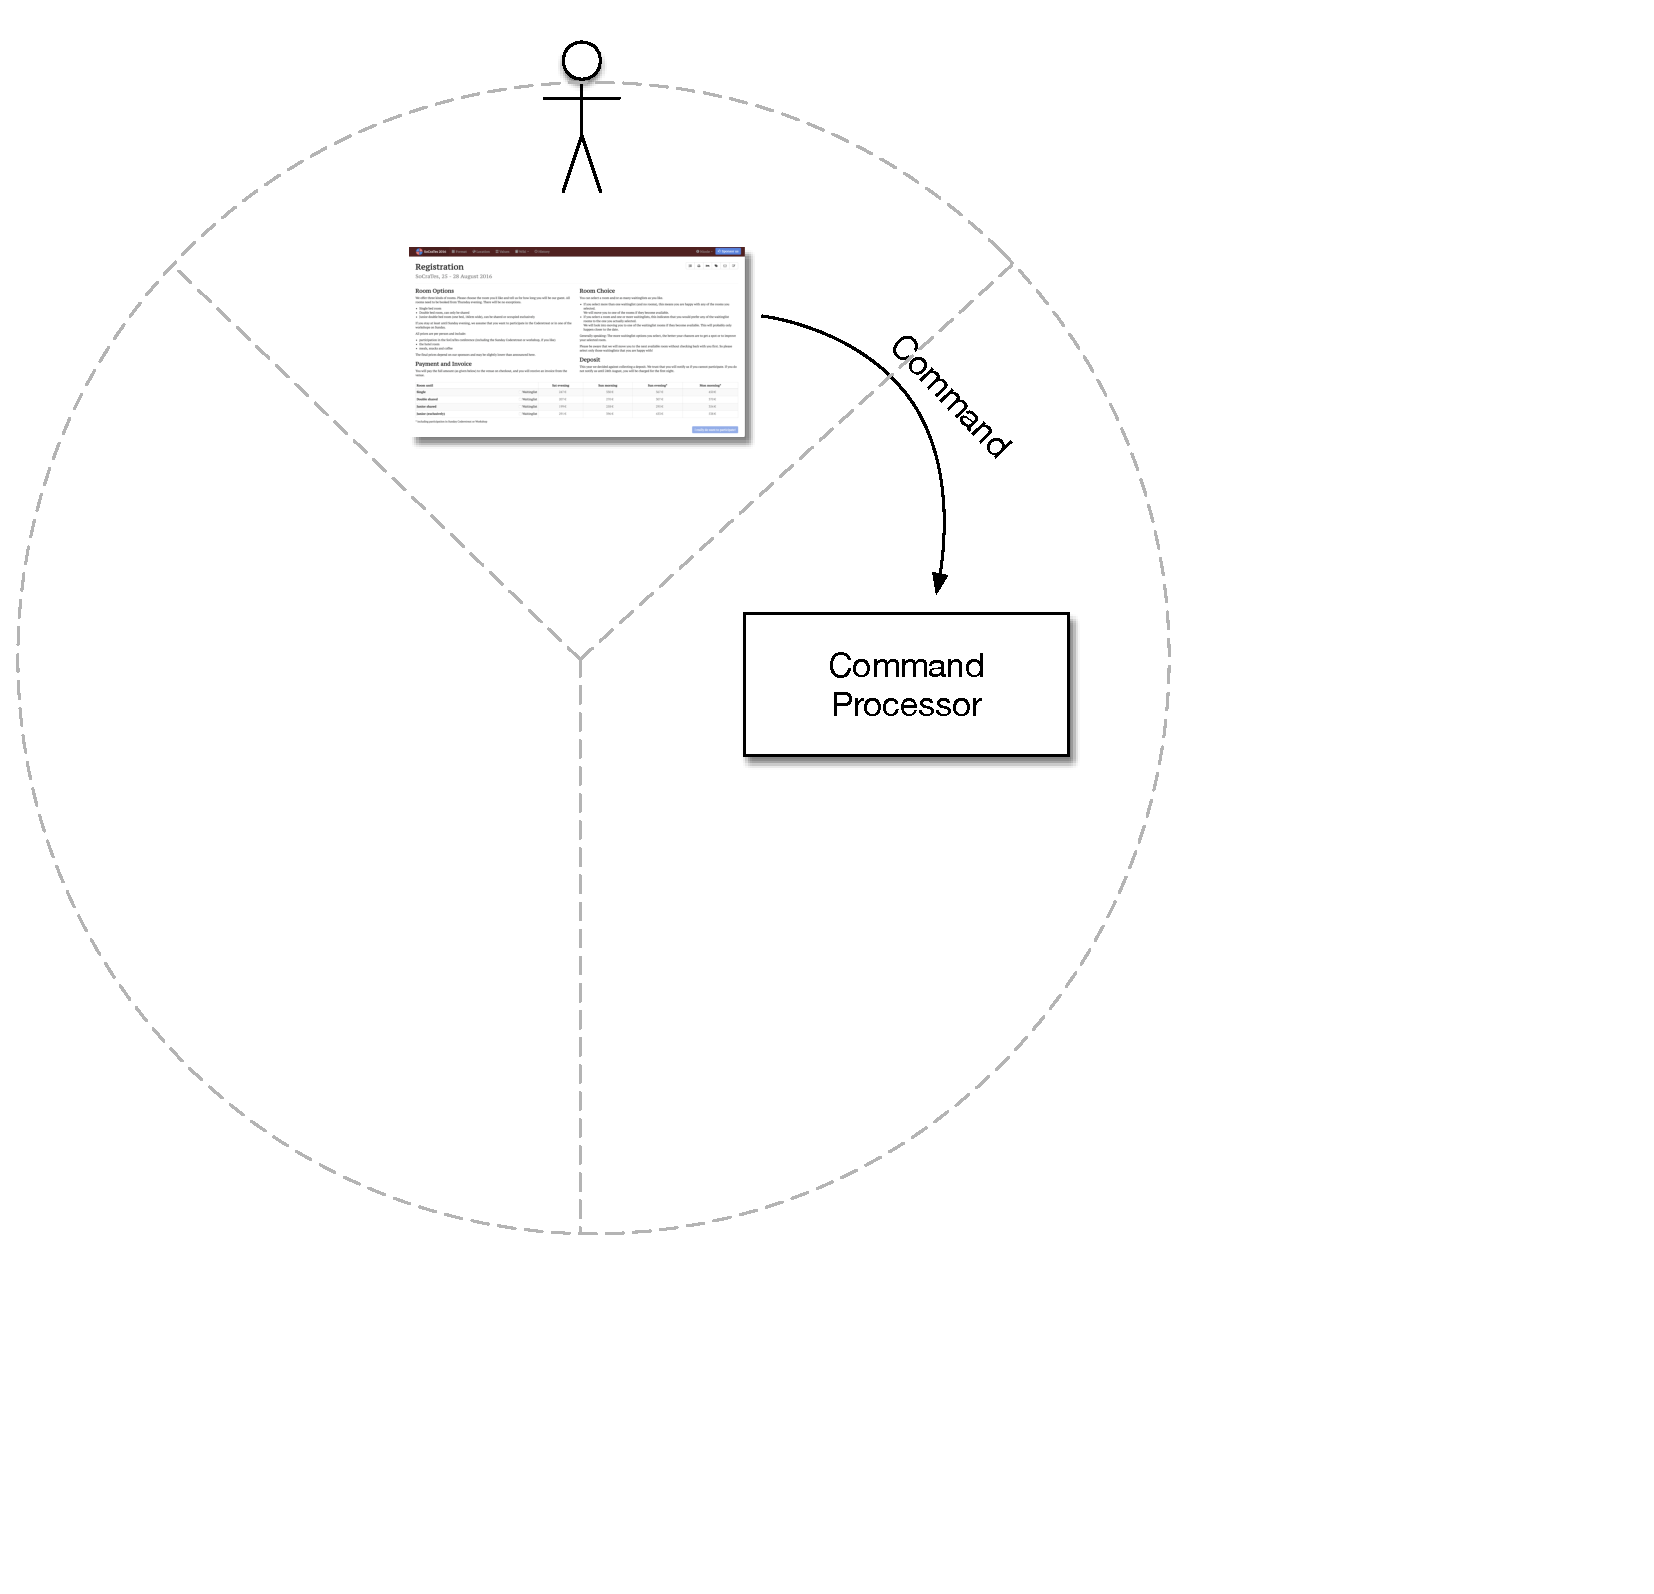
\includegraphics[width=.7\textwidth]{../EventSourcing1.pdf}
\end{onlyenv}

\begin{onlyenv}<2>
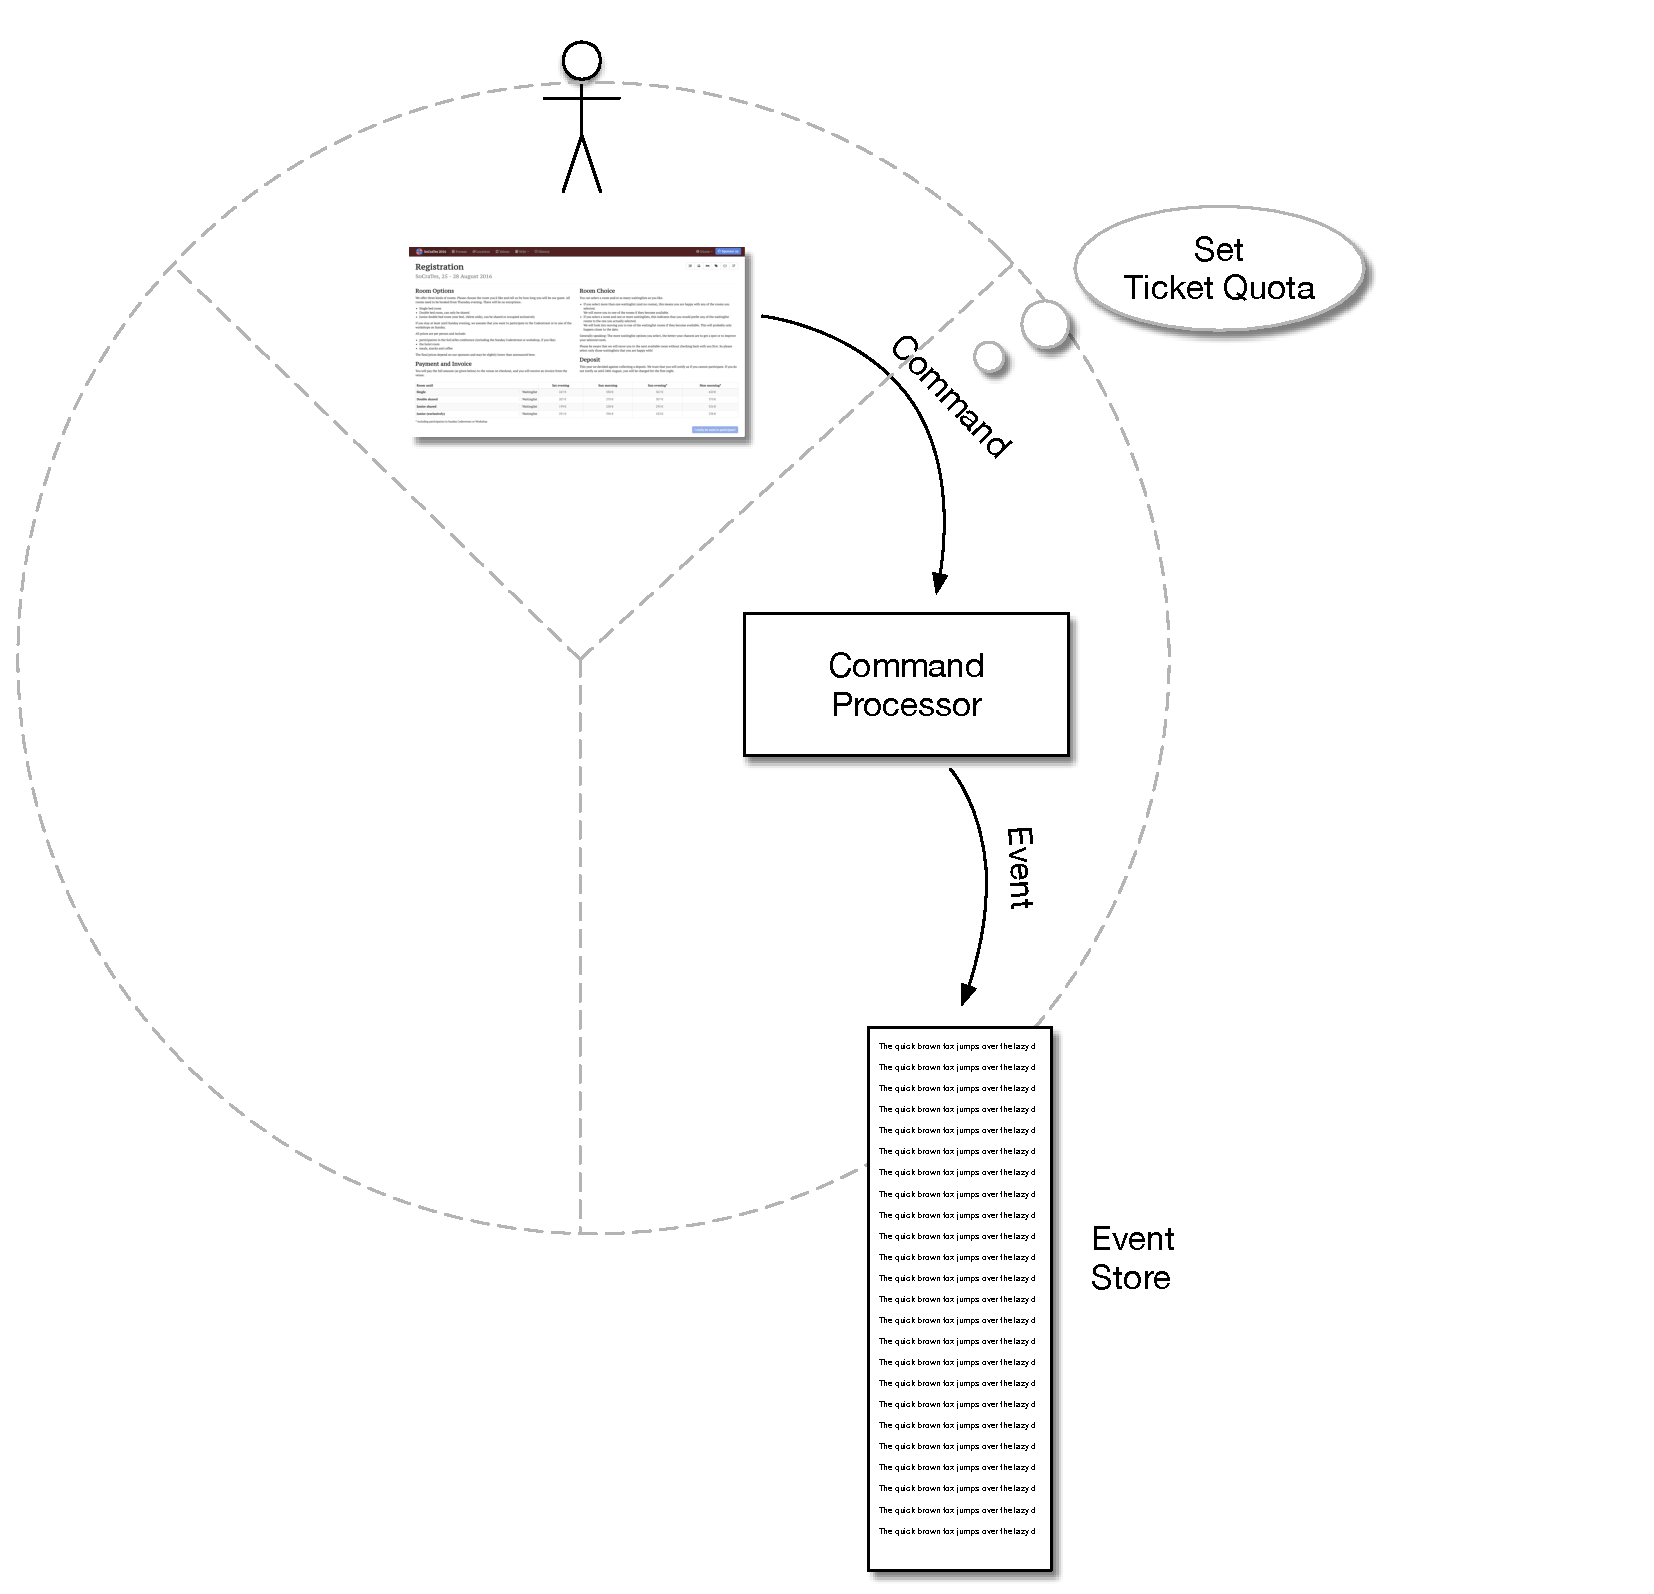
\includegraphics[width=.7\textwidth]{../EventSourcing2.pdf}
\end{onlyenv}

\begin{onlyenv}<3-4>
\begin{minipage}{.7\textwidth}
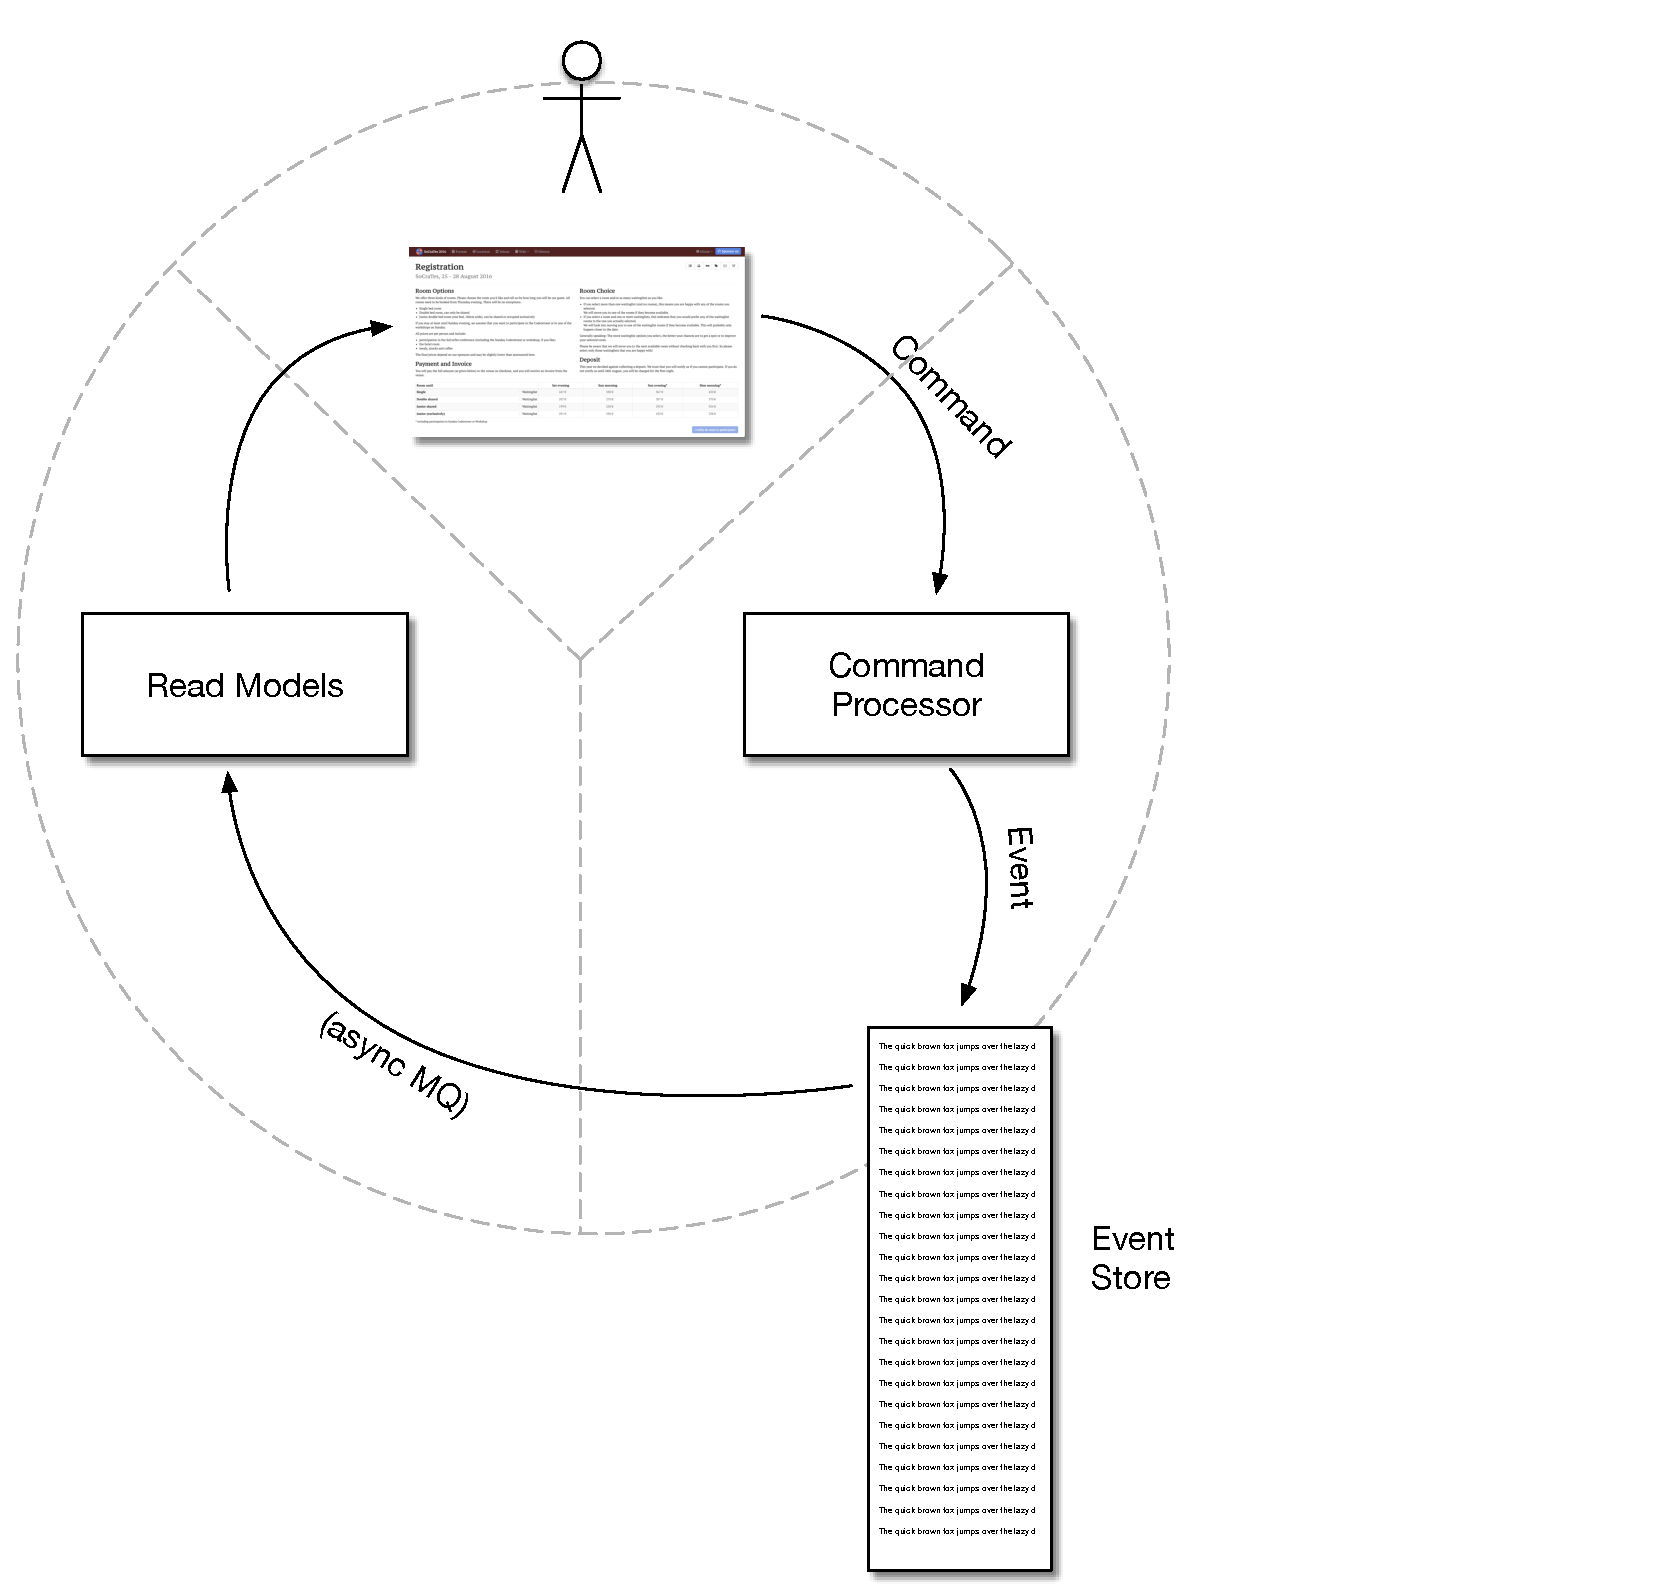
\includegraphics[width=\textwidth]{../EventSourcing3.pdf}
\end{minipage} \hfill
\end{onlyenv}
\begin{onlyenv}<3>
\begin{minipage}{0.25\textwidth}
\small
Set ticket count
\begin{itemize}
\item Ticket count set
\end{itemize}
\end{minipage}
\end{onlyenv}
\begin{onlyenv}<4>
\begin{minipage}{0.25\textwidth}
\small
Book ticket
\begin{itemize}
\item Ticket booked
\item Sold out
\item You already booked a ticket
\end{itemize}
\end{minipage}
\end{onlyenv}

\begin{onlyenv}<5>
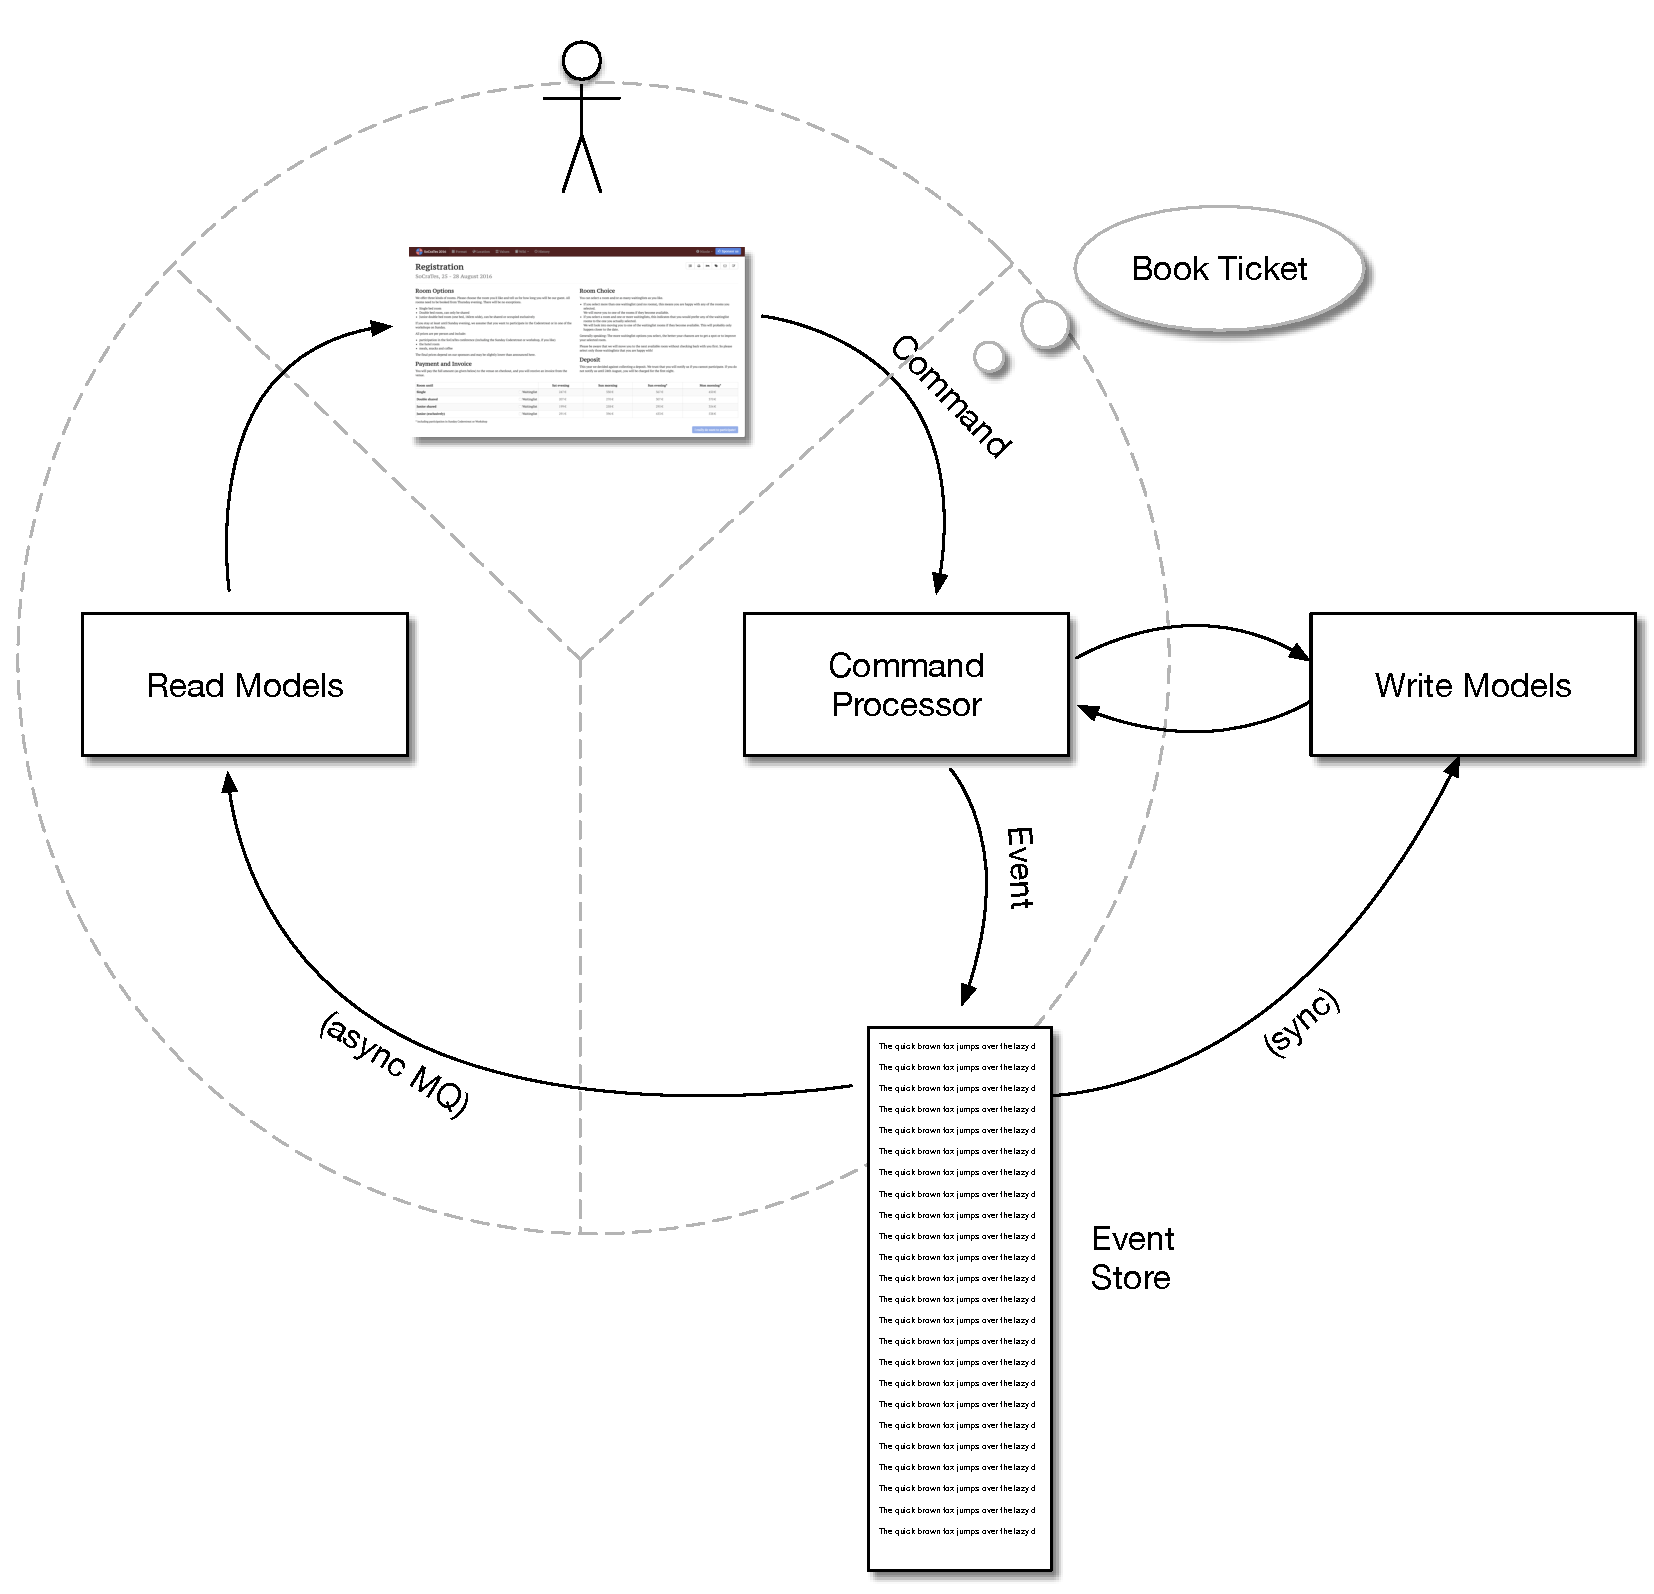
\includegraphics[width=.7\textwidth]{../EventSourcing4.pdf}
\end{onlyenv}

\end{frame}

%%%%%%%%%%%%%%%%%%%%%%%%%%%%%%%%%%%%%%%%%%%%%%%%%%
\begin{frame}[fragile]{Standard Event Sourcing Scenario}

\begin{itemize}
\item Event sourcing in application server
\item Incremental updates of event store, write models and read models
\item Write models must be updated synchronously
\item Read models can be updated asynchronously
\end{itemize}

\end{frame}

%%%%%%%%%%%%%%%%%%%%%%%%%%%%%%%%%%%%%%%%%%%%%%%%%%
\begin{frame}[fragile]{Event Sourcing in Node.js}

Let's understand how node.js works

\end{frame}

%%%%%%%%%%%%%%%%%%%%%%%%%%%%%%%%%%%%%%%%%%%%%%%%%%
\begin{frame}[fragile]{Node.js}

\begin{onlyenv}<1>
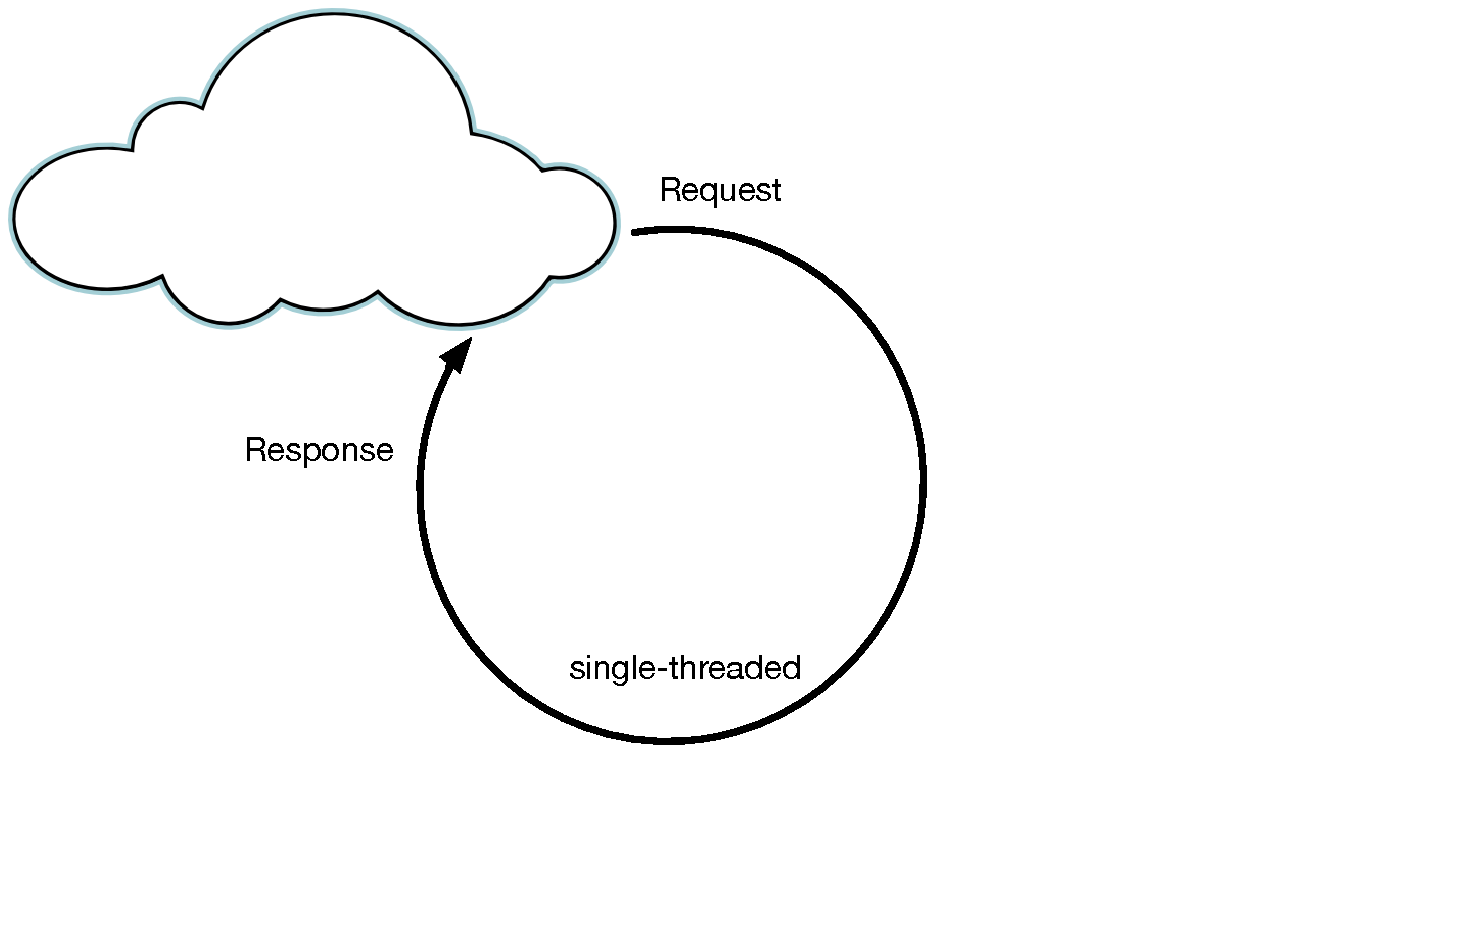
\includegraphics[width=.7\textwidth]{../Nodejs1.pdf}
\end{onlyenv}

\begin{onlyenv}<2>
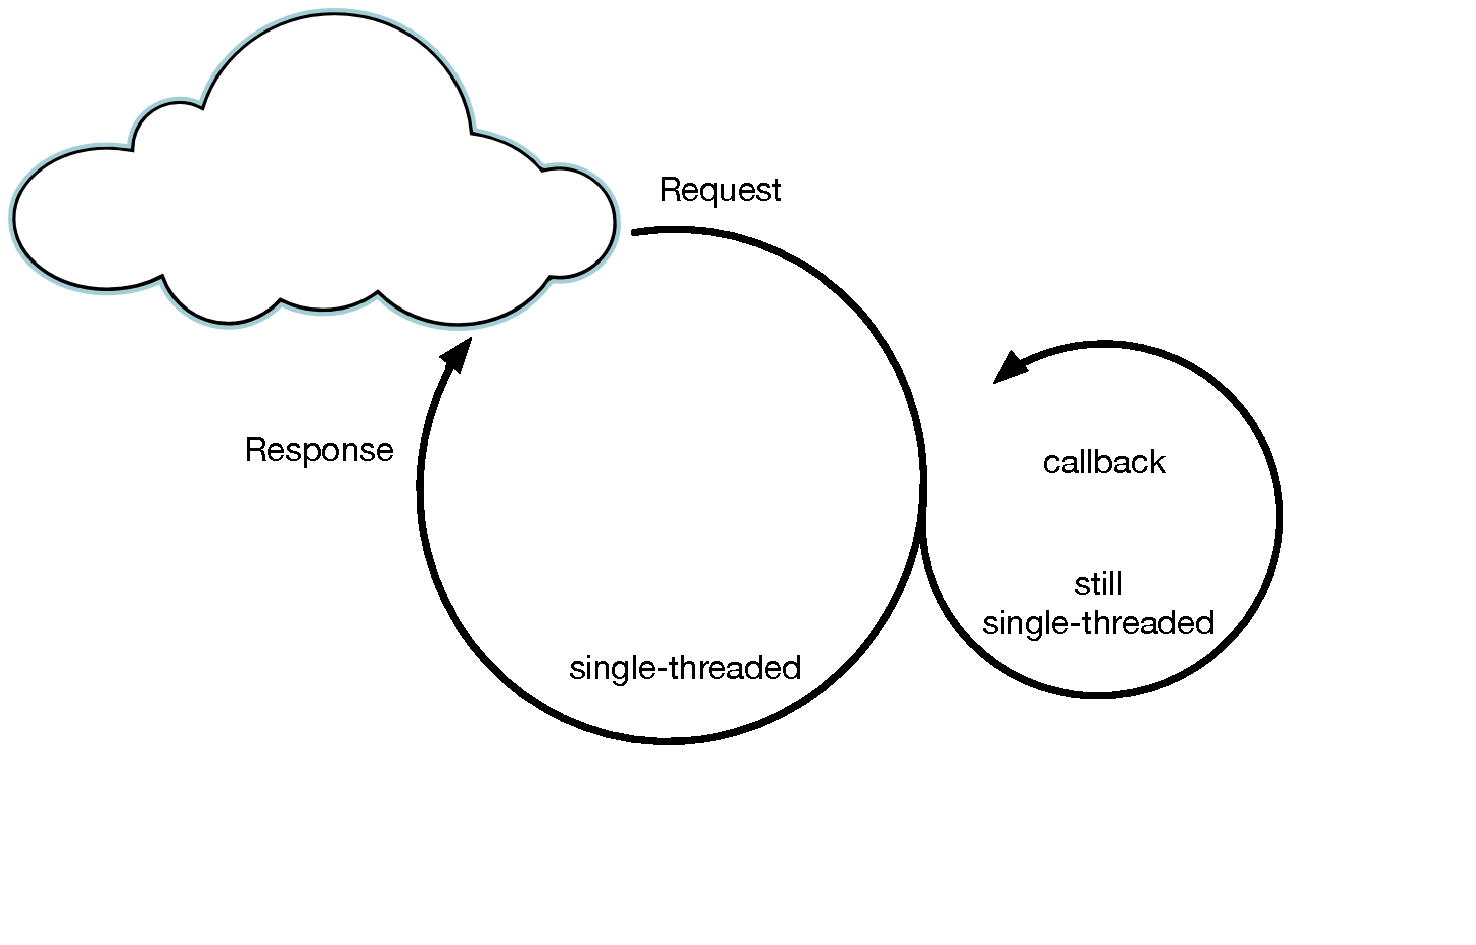
\includegraphics[width=.7\textwidth]{../Nodejs2.pdf}
\end{onlyenv}

\begin{onlyenv}<3>
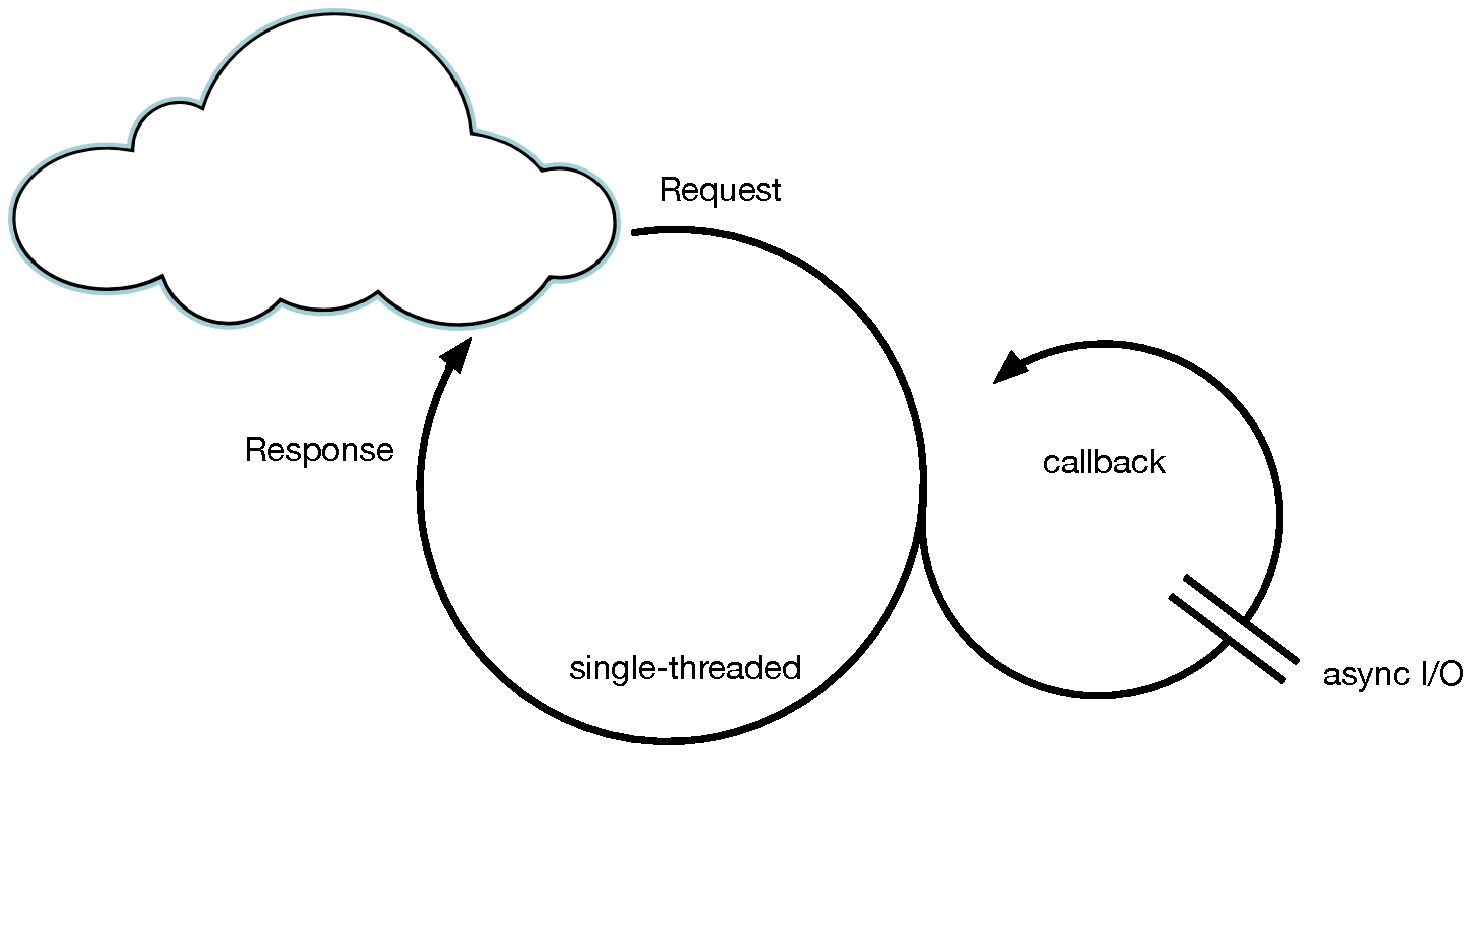
\includegraphics[width=.7\textwidth]{../Nodejs3.pdf}
\end{onlyenv}

\begin{onlyenv}<4>
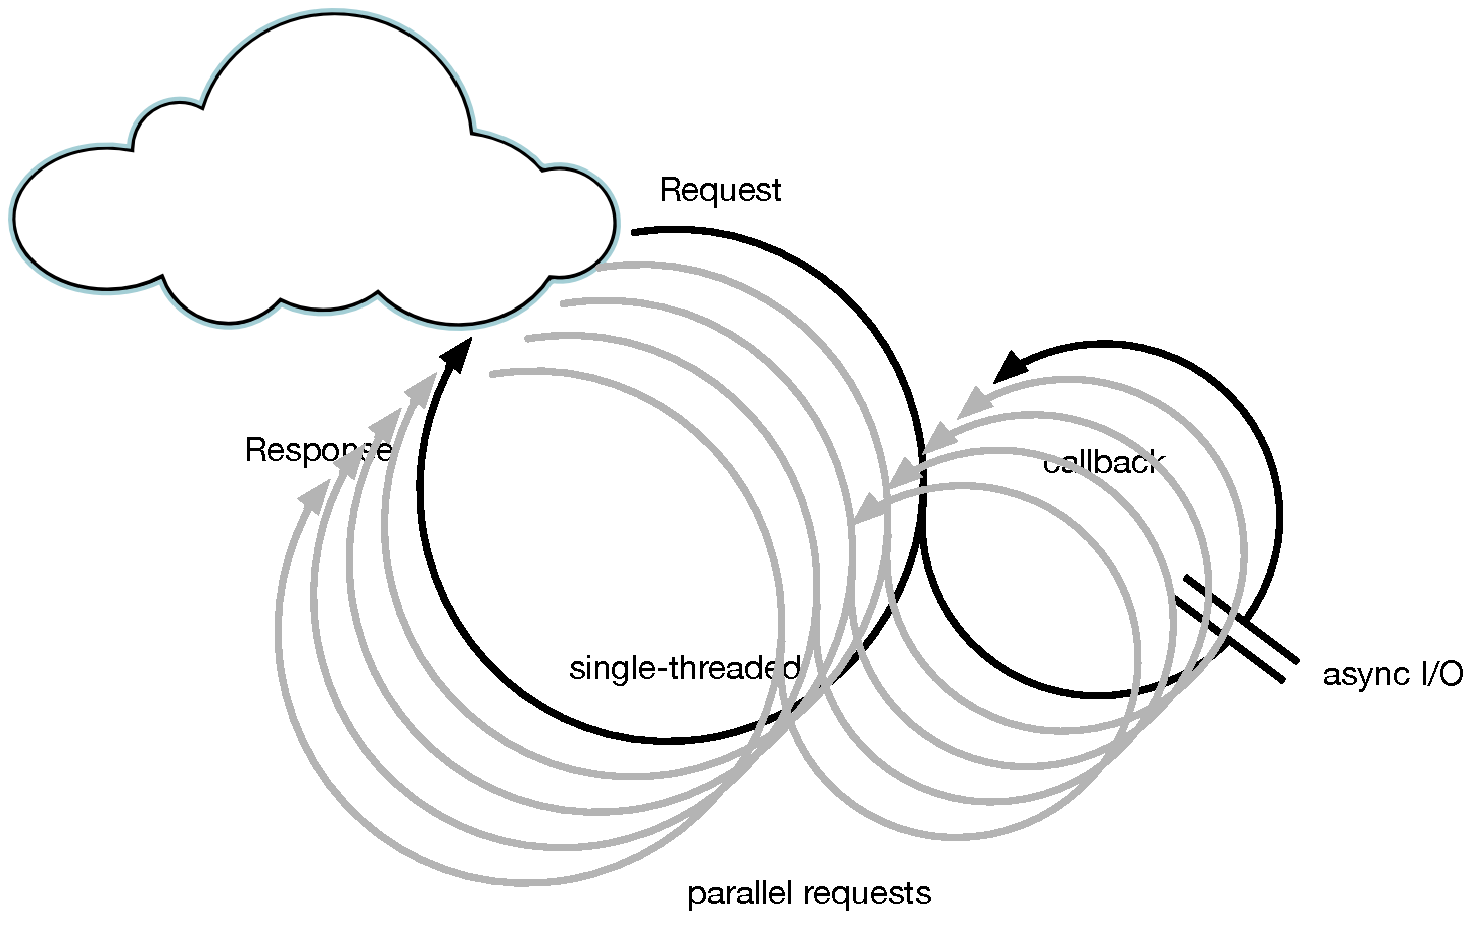
\includegraphics[width=.7\textwidth]{../Nodejs4.pdf}
\end{onlyenv}

\hfill 

\begin{tiny}
\makebox[\textwidth][r]{\url{http://blog.mixu.net/2011/02/01/understanding-the-node-js-event-loop/}}
\end{tiny}

\end{frame}

%%%%%%%%%%%%%%%%%%%%%%%%%%%%%%%%%%%%%%%%%%%%%%%%%%
\begin{frame}[fragile]{Mongo DB}

\begin{itemize}
\item No transactions
\item No optimistic locking
\onslide+<2->
\item We implemented optimistic locking ourselves
\end{itemize}

\end{frame}

%%%%%%%%%%%%%%%%%%%%%%%%%%%%%%%%%%%%%%%%%%%%%%%%%%
\begin{frame}[fragile]{Mongo DB}

\begin{center}

\begin{onlyenv}<1>
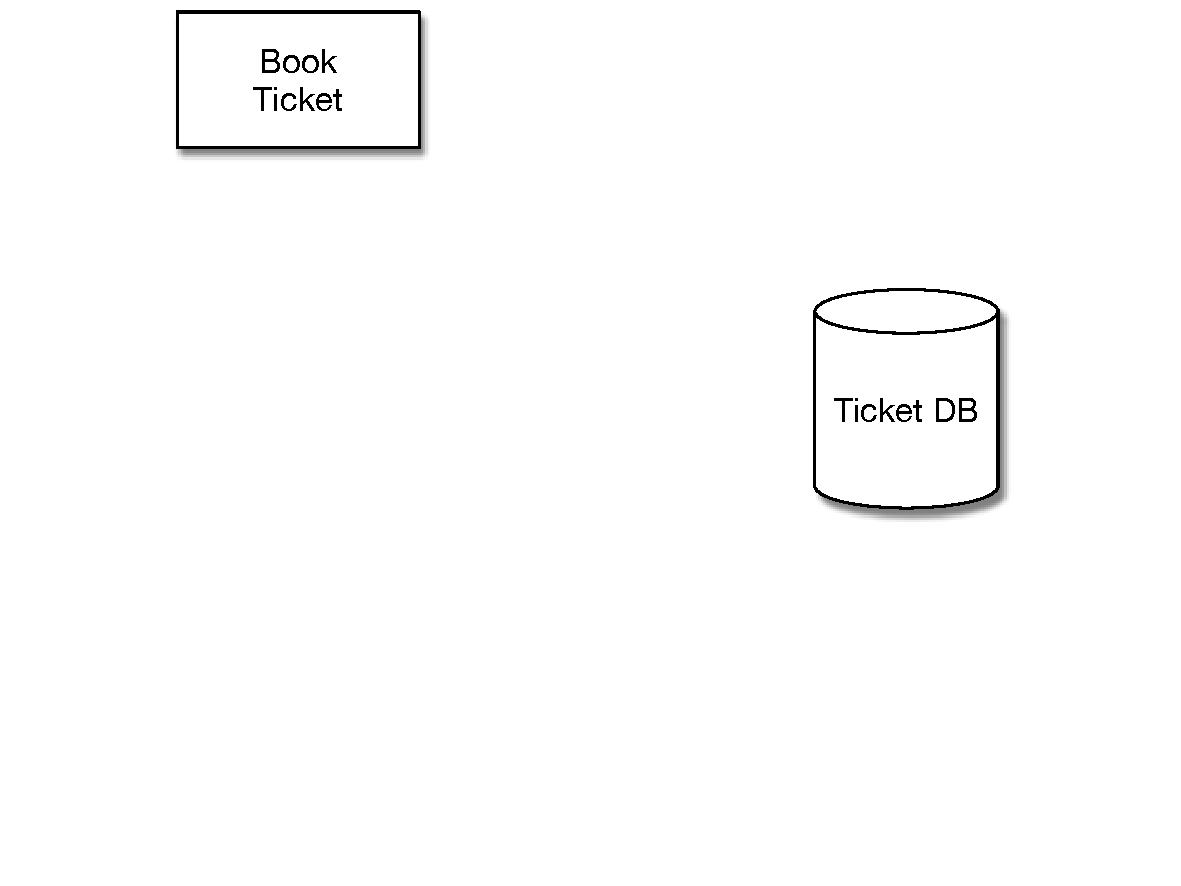
\includegraphics[width=.85\textwidth]{../OptimisticLocking1.pdf}
\end{onlyenv}

\begin{onlyenv}<2>
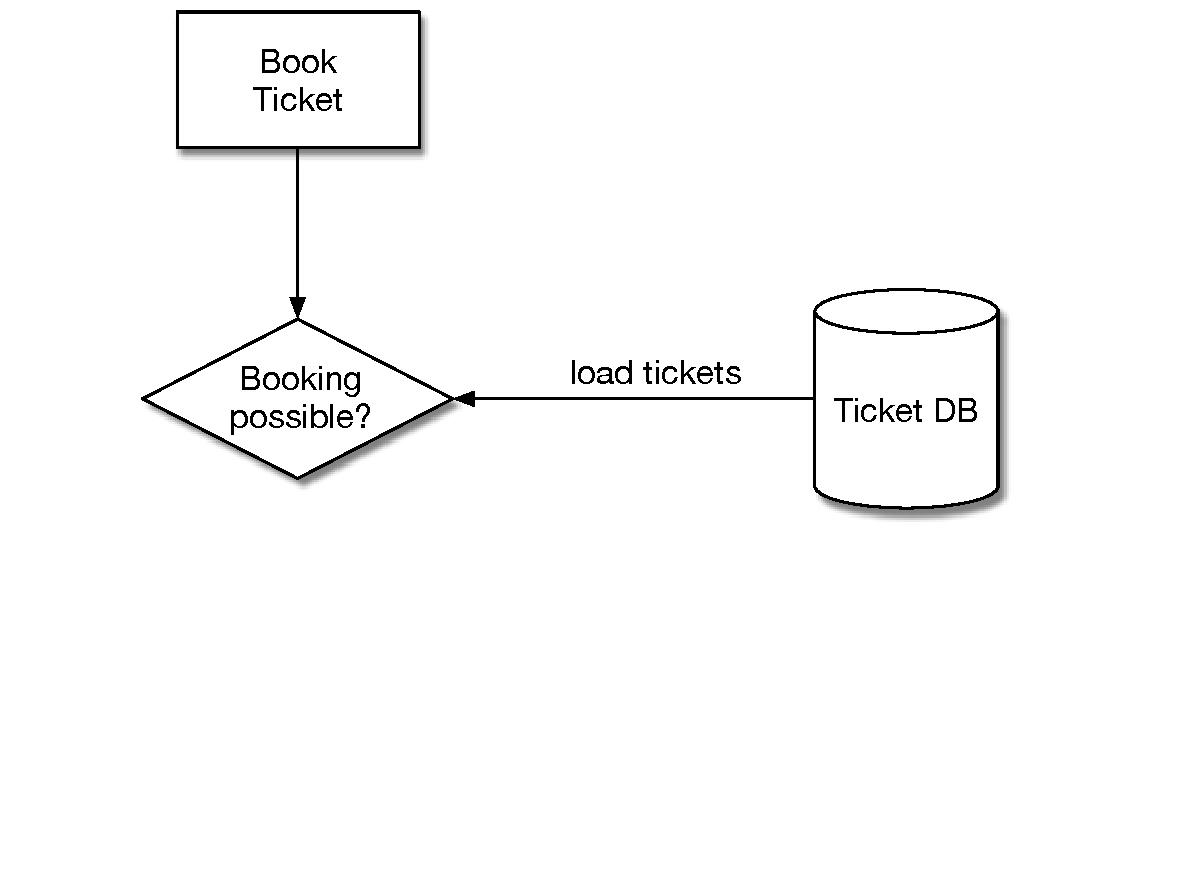
\includegraphics[width=.85\textwidth]{../OptimisticLocking2.pdf}
\end{onlyenv}

\begin{onlyenv}<3>
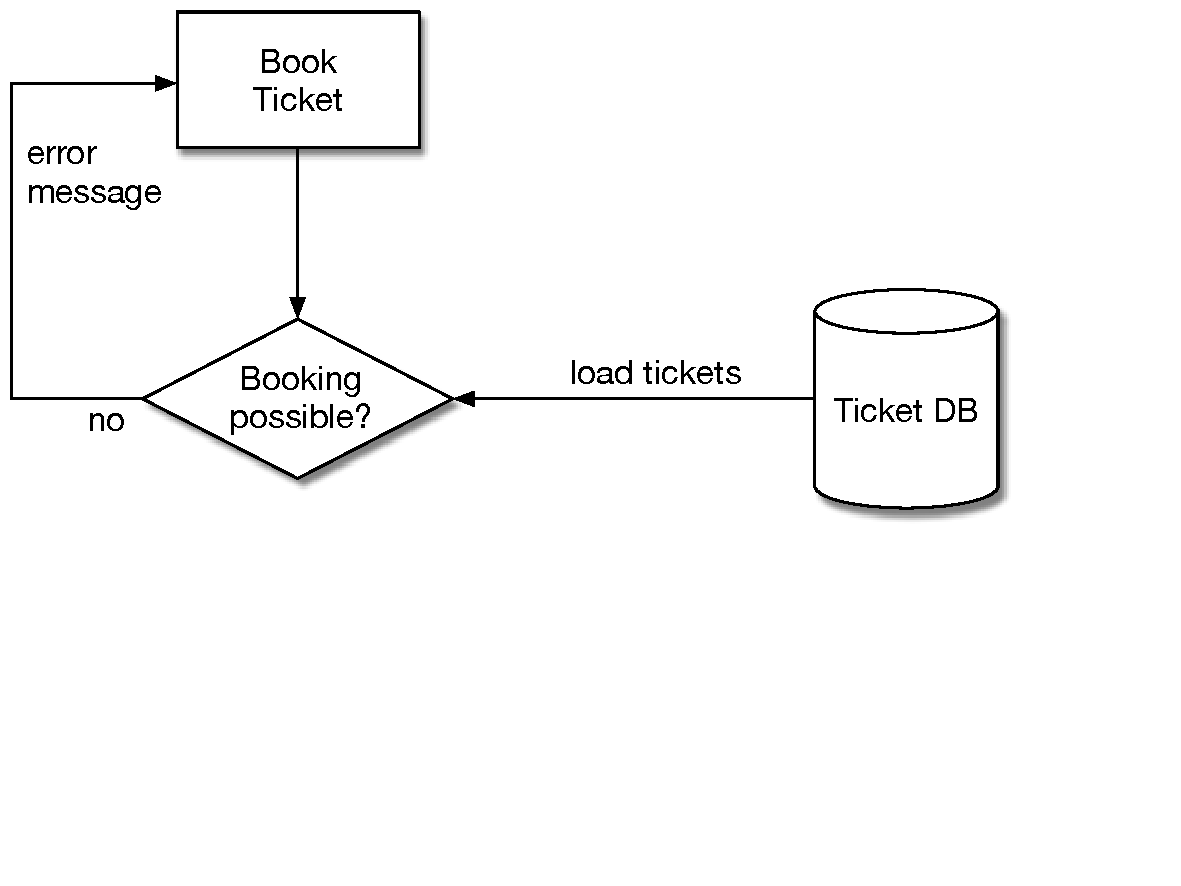
\includegraphics[width=.85\textwidth]{../OptimisticLocking3.pdf}
\end{onlyenv}

\begin{onlyenv}<4>
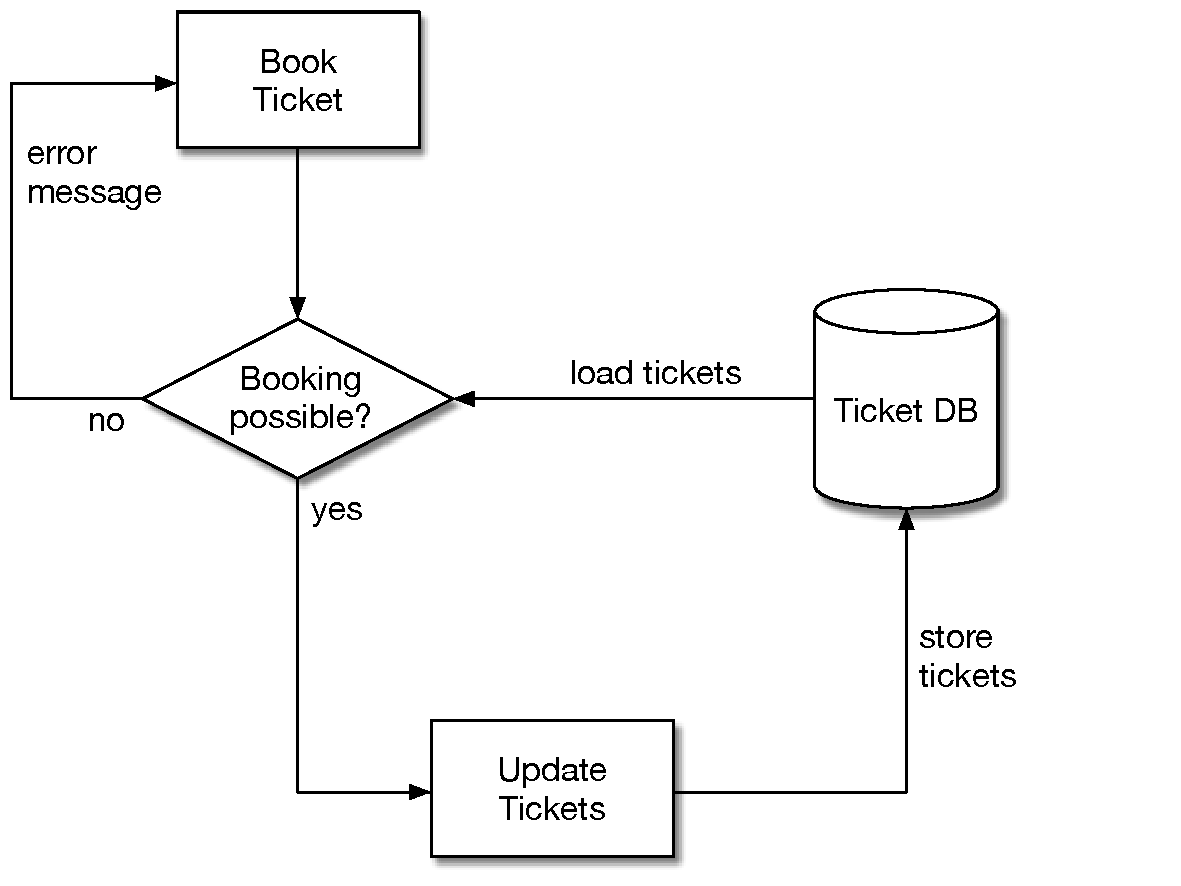
\includegraphics[width=.85\textwidth]{../OptimisticLocking4.pdf}
\end{onlyenv}

\begin{onlyenv}<5>
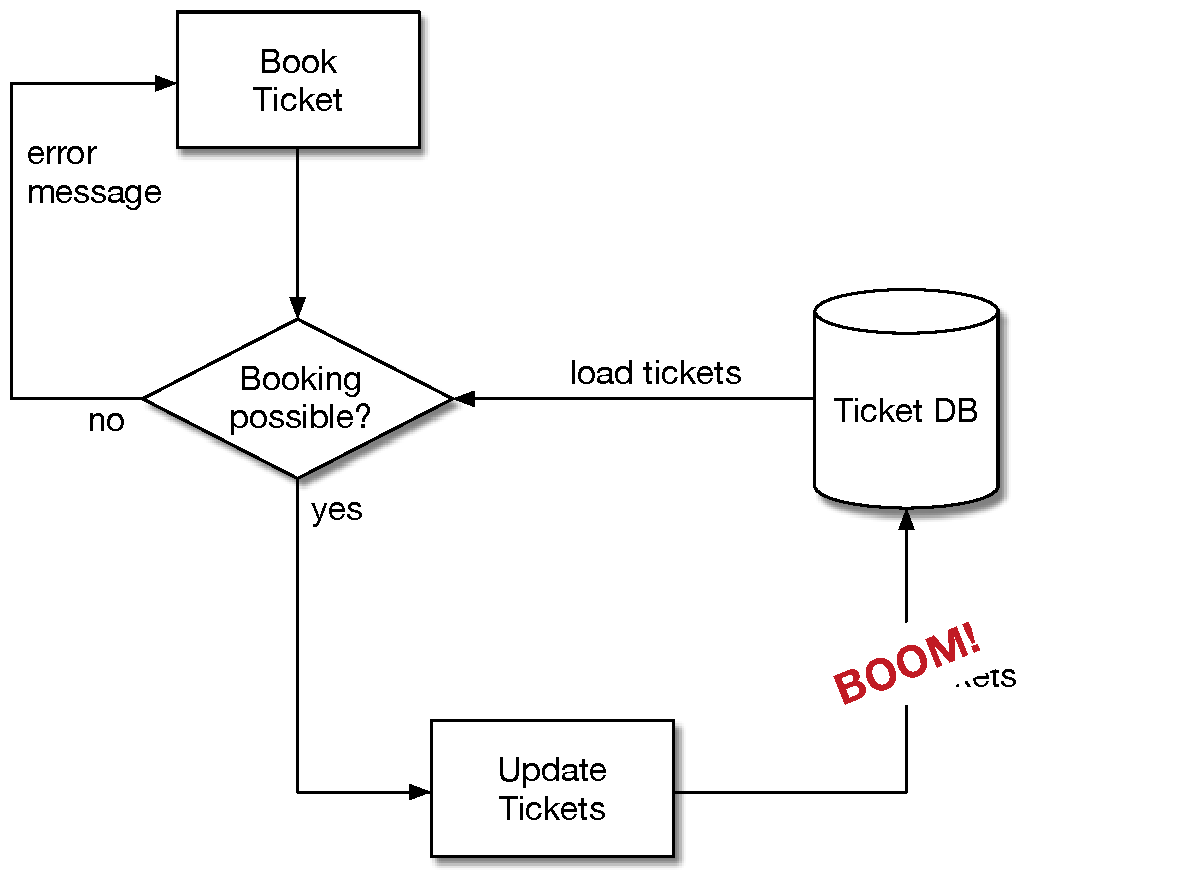
\includegraphics[width=.85\textwidth]{../OptimisticLocking5.pdf}
\end{onlyenv}

\begin{onlyenv}<6>
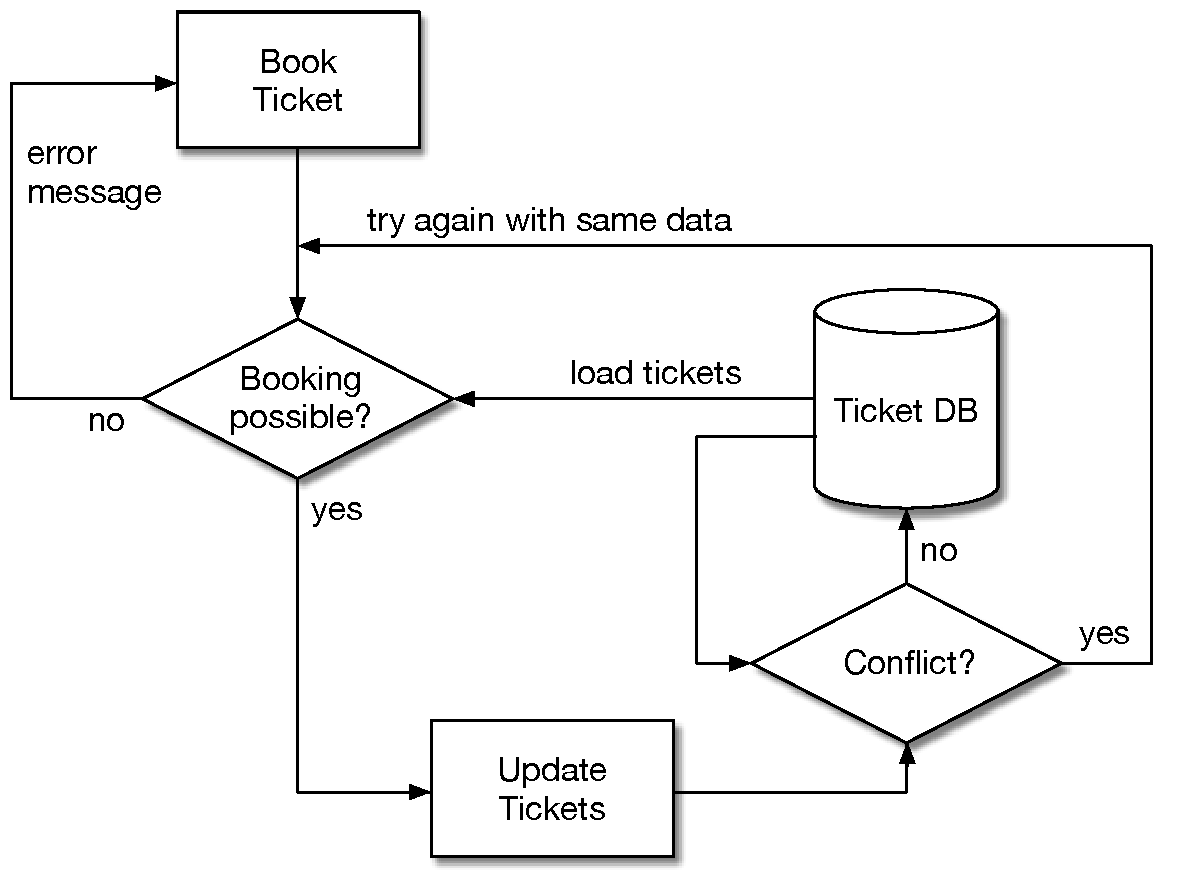
\includegraphics[width=.85\textwidth]{../OptimisticLocking6.pdf}
\end{onlyenv}

\end{center}

\end{frame}

%%%%%%%%%%%%%%%%%%%%%%%%%%%%%%%%%%%%%%%%%%%%%%%%%%
\begin{frame}[fragile]{Our Initial Architecture}

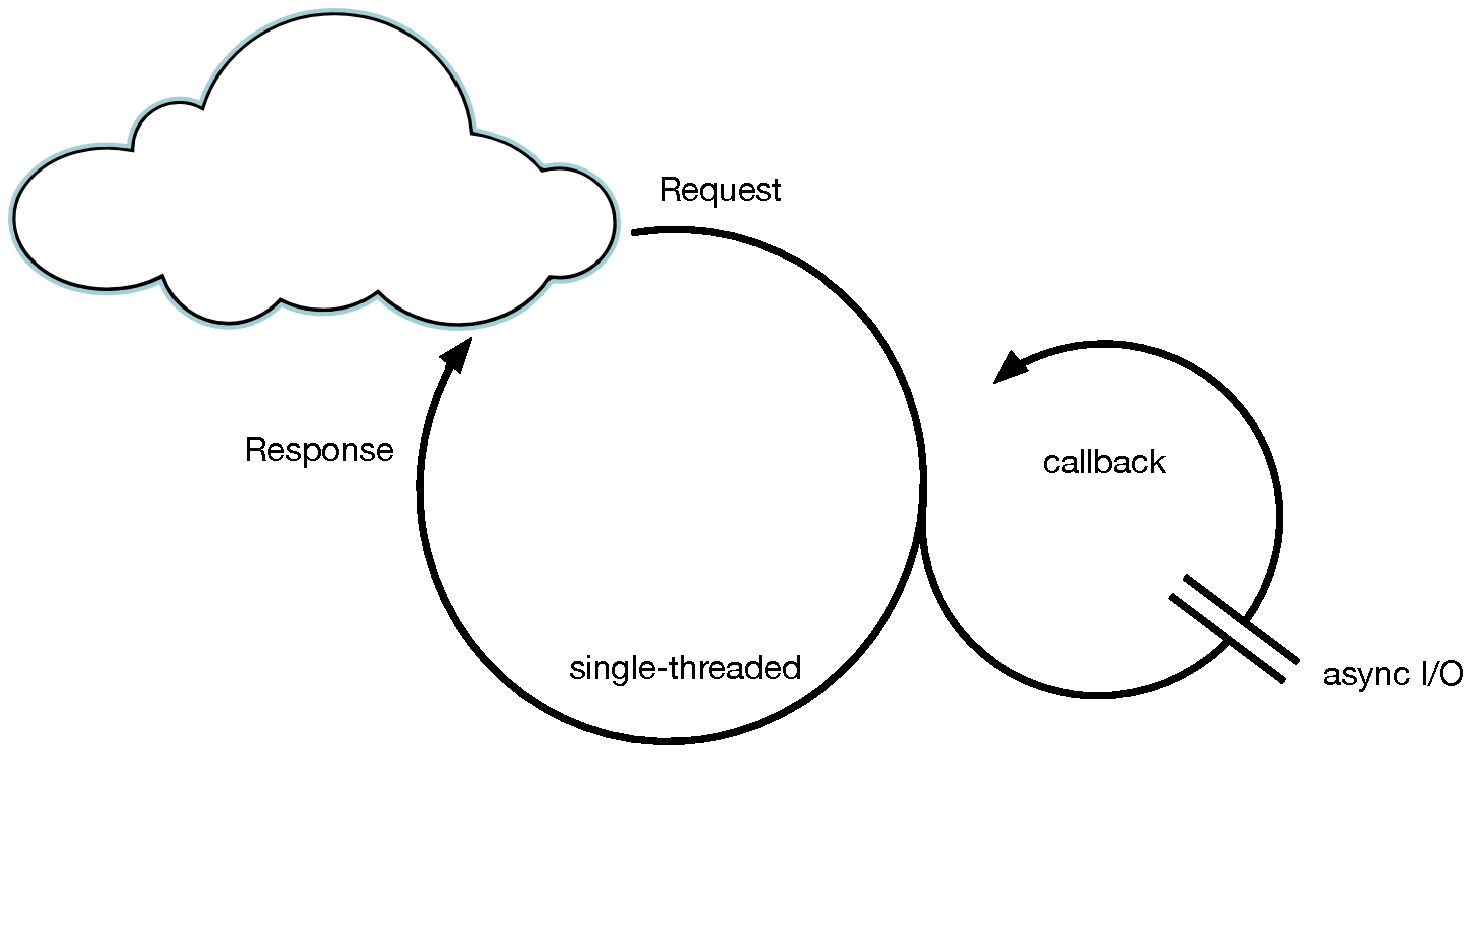
\includegraphics[width=.7\textwidth]{../Nodejs3.pdf}

\onslide+<2->

\begin{itemize}
\item Request comes in, reads \& writes data from/to DB, returns
\item Nothing$^*$ is kept in memory between requests
\end{itemize}

{ \tiny $^*$ Apart from the caching that is done by \texttt{require} }
\end{frame}

%%%%%%%%%%%%%%%%%%%%%%%%%%%%%%%%%%%%%%%%%%%%%%%%%%
\begin{frame}[fragile]{Event Sourcing Without Global State?}

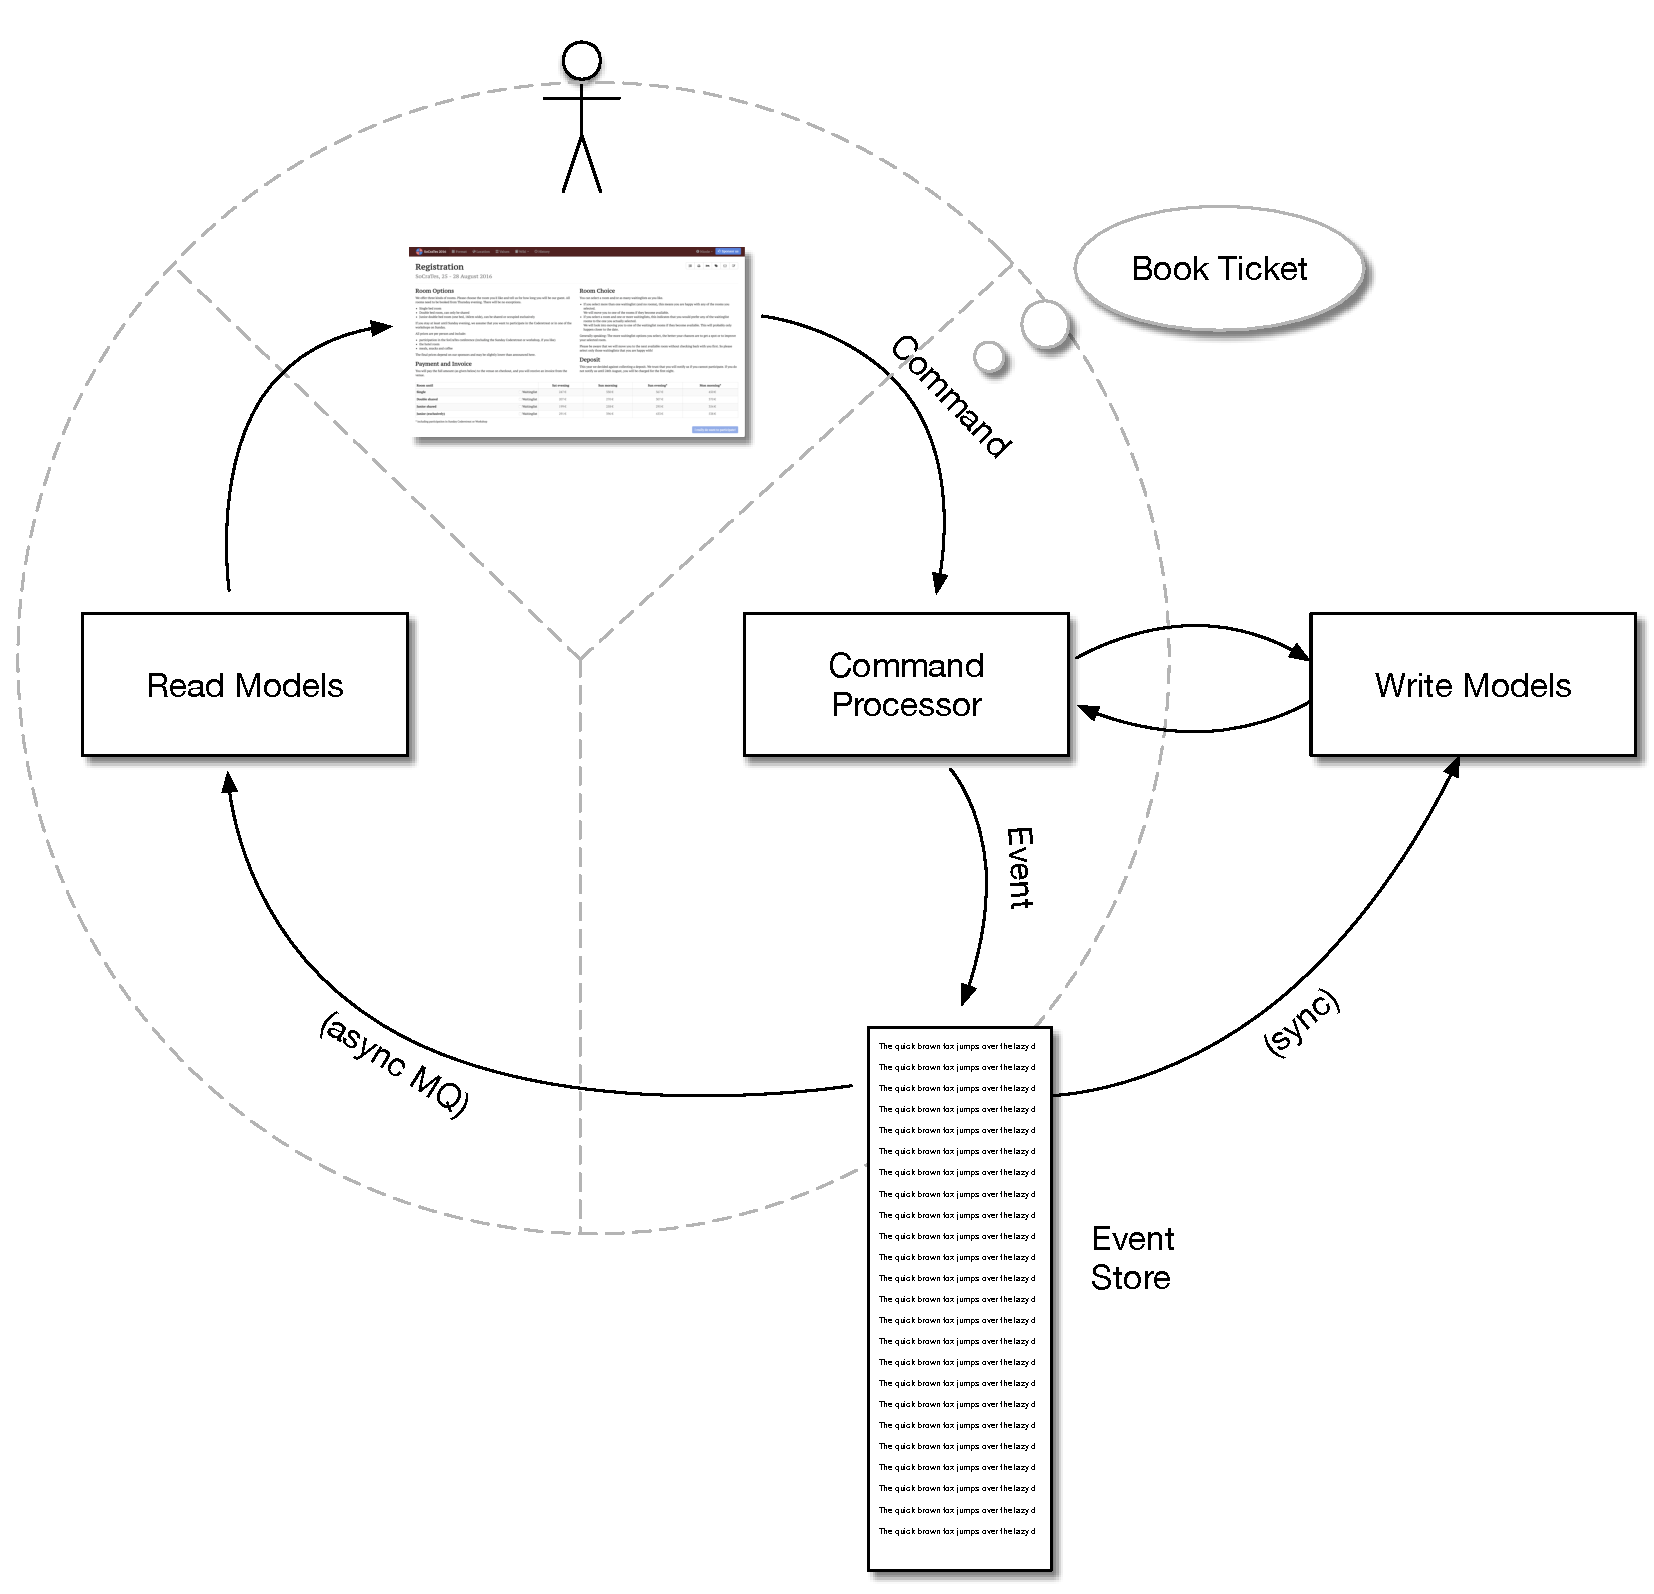
\includegraphics[width=.5\textwidth]{../EventSourcing4.pdf}

\onslide+<2->

\begin{itemize}
\item What about the read and write models?
\end{itemize}

\end{frame}

%%%%%%%%%%%%%%%%%%%%%%%%%%%%%%%%%%%%%%%%%%%%%%%%%%
\begin{frame}[fragile]{Working Hypothesis}

\textbf{Rough Estimations:} \\[.7em]
We expected a couple hundred events altogether

\onslide+<2->
\vspace{5em}

\textbf{Working Hypothesis:} \\[.7em]
We can hydrate the models from the event store on each request

\end{frame}


%%%%%%%%%%%%%%%%%%%%%%%%%%%%%%%%%%%%%%%%%%%%%%%%%%
\begin{frame}[fragile]{On Opening the Registration}

\onslide+<2->

Registration began...

\onslide+<3->

\vspace{3em}

~ \hspace{10em} ... but nobody registered!
 
\end{frame}

%%%%%%%%%%%%%%%%%%%%%%%%%%%%%%%%%%%%%%%%%%%%%%%%%%
\begin{frame}[fragile]{What was going on?}

Remember: 2-phase registration (reservation -> registration)

First user came in:

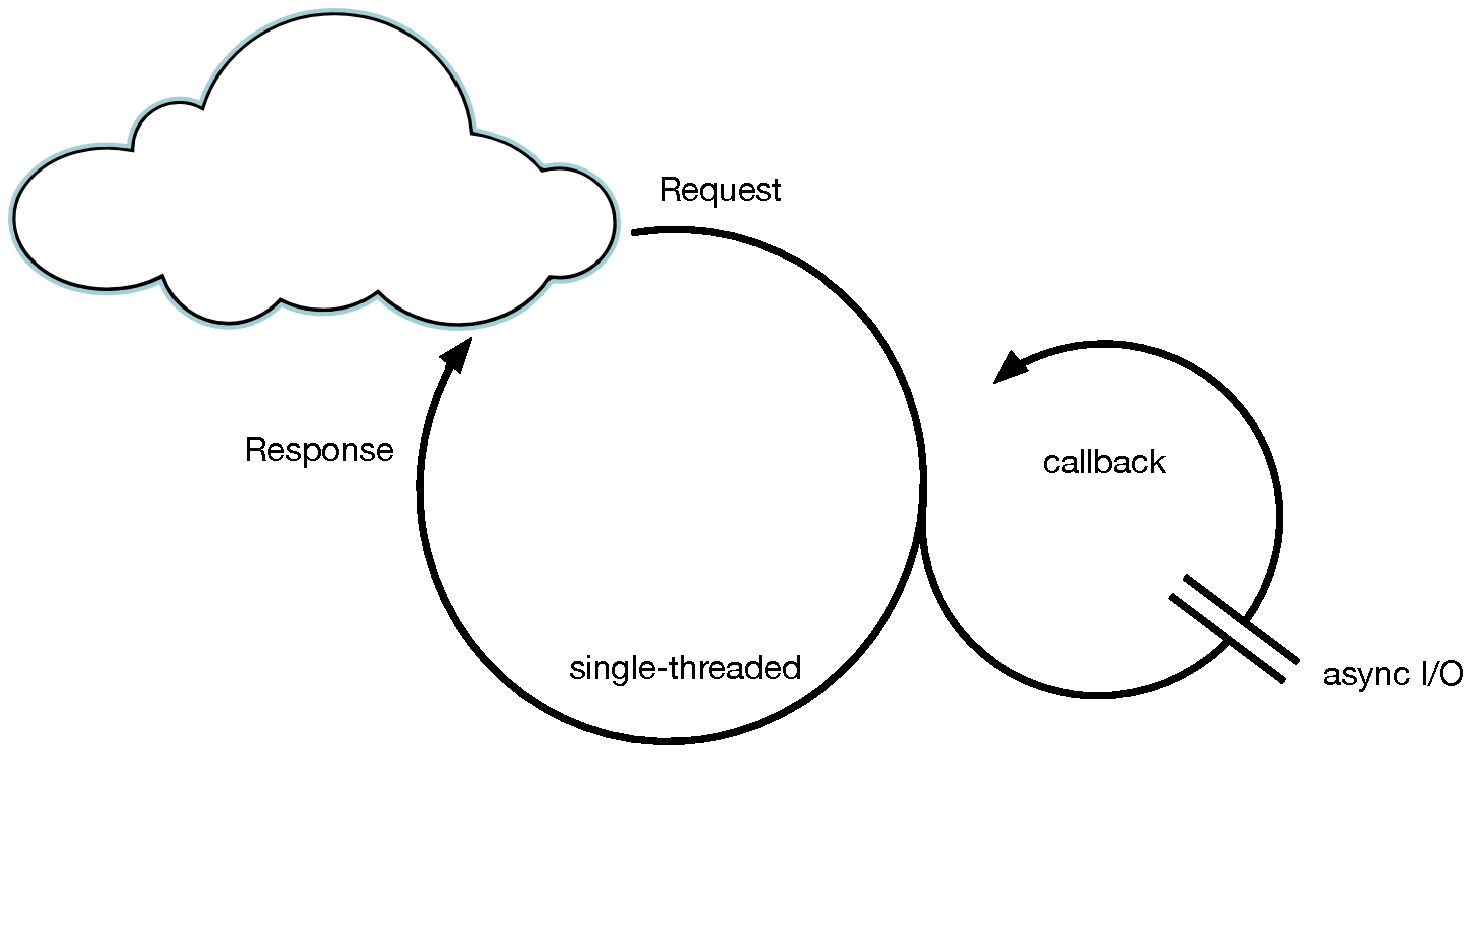
\includegraphics[width=.4\textwidth]{../Nodejs3.pdf}

Reading from DB parallelized it, so more users came in and read from DB

\end{frame}

%%%%%%%%%%%%%%%%%%%%%%%%%%%%%%%%%%%%%%%%%%%%%%%%%%
\begin{frame}[fragile]{What was going on?}

First user was able to persist her reservation:

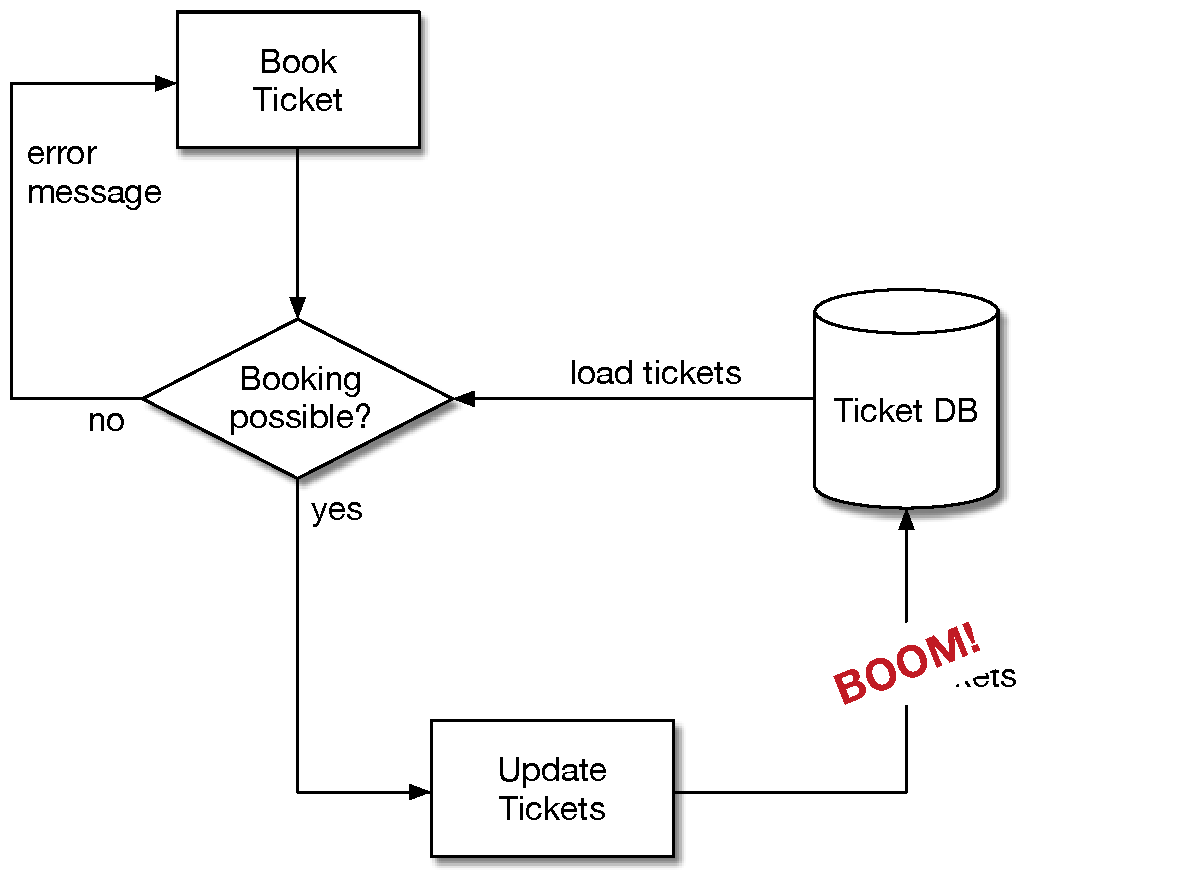
\includegraphics[width=.4\textwidth]{../OptimisticLocking5.pdf}

All subsequent users produced conflicts: 

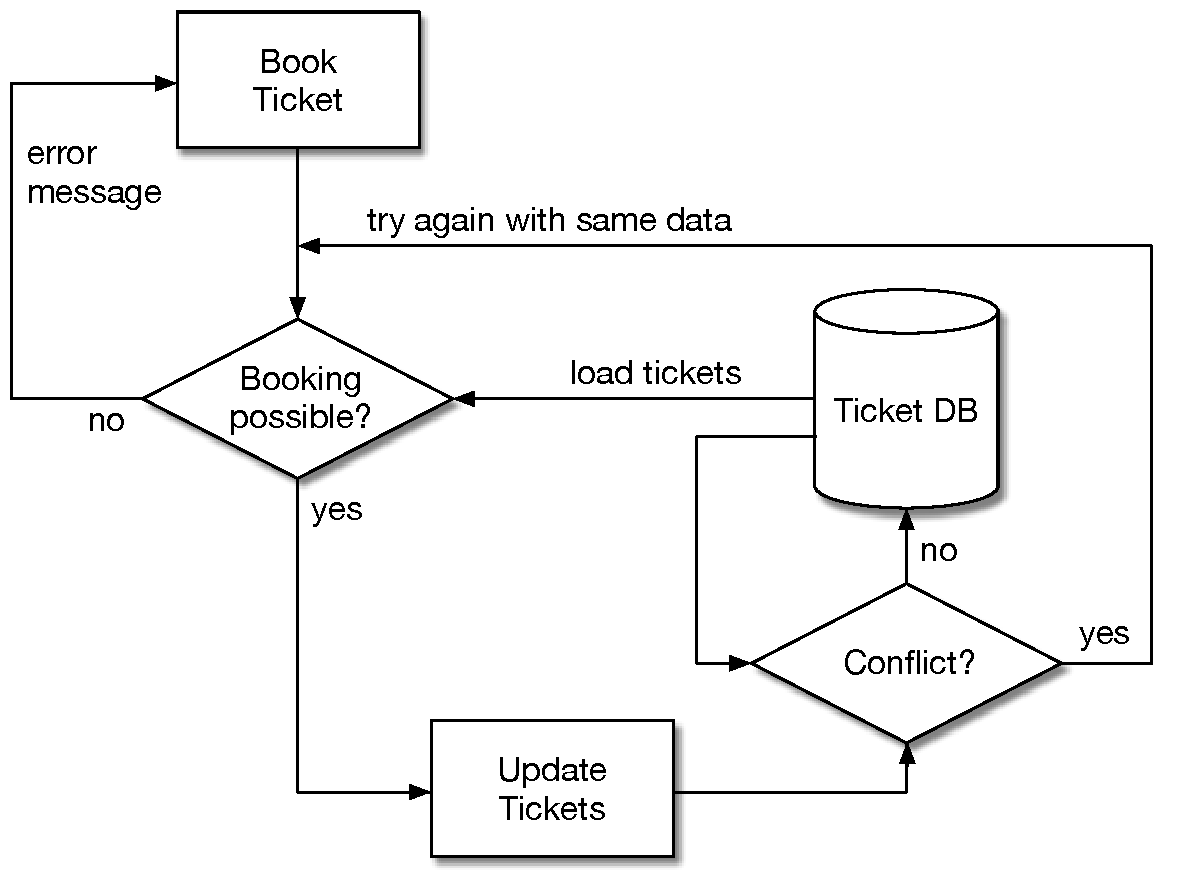
\includegraphics[width=.4\textwidth]{../OptimisticLocking6.pdf}

And retried.

And got conflicts again.

And retried again.

\end{frame}

%%%%%%%%%%%%%%%%%%%%%%%%%%%%%%%%%%%%%%%%%%%%%%%%%%
\begin{frame}[fragile]{}

Because in fact it was

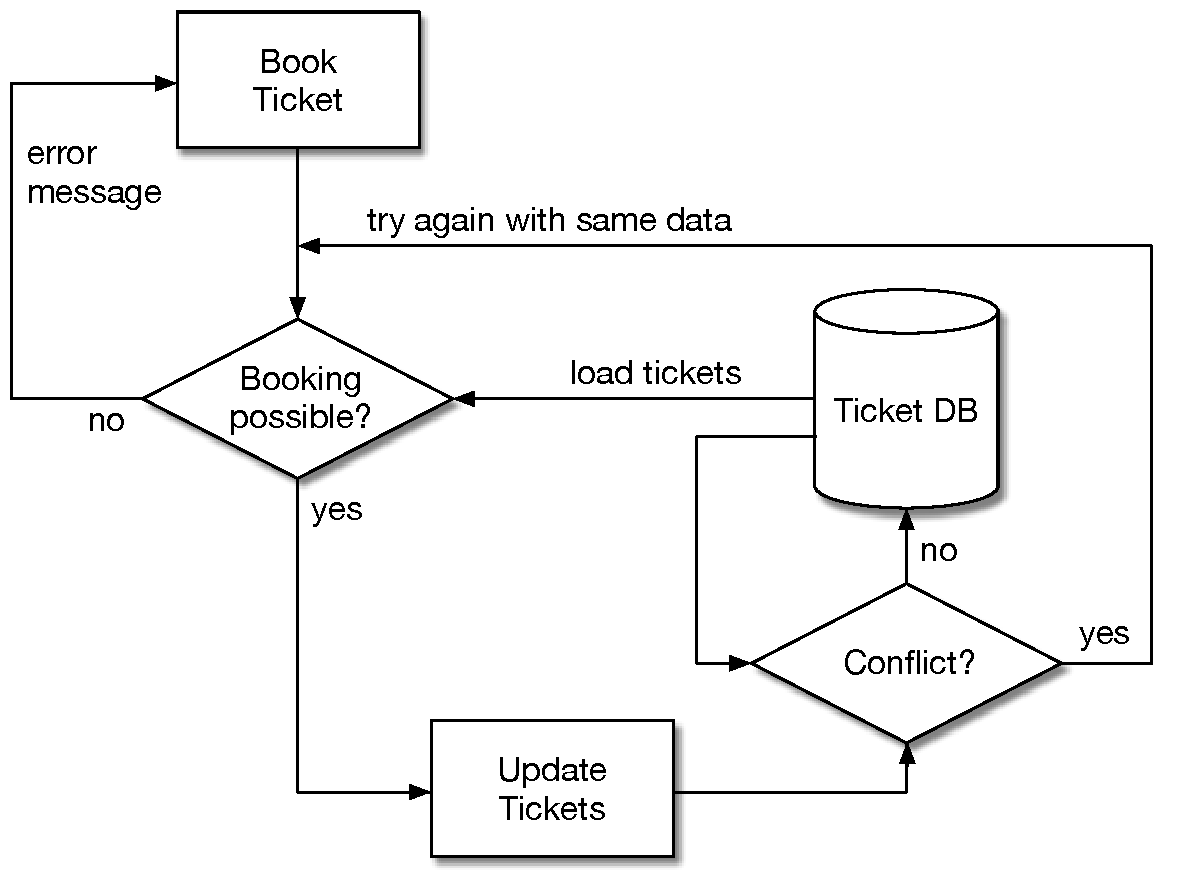
\includegraphics[width=.4\textwidth]{../OptimisticLocking6.pdf}

so we had a self-propelling disaster.

\end{frame}

%%%%%%%%%%%%%%%%%%%%%%%%%%%%%%%%%%%%%%%%%%%%%%%%%%
\begin{frame}[fragile]{The End}

After 25 minutes, I shut down the server.
                  
\onslide+<2->
                  
\vspace{3em}

~ \hspace{10em} Nobody had been able to register.
                  
\end{frame}

%%%%%%%%%%%%%%%%%%%%%%%%%%%%%%%%%%%%%%%%%%%%%%%%%%
\begin{frame}[fragile]{Problem I}

Hydrating the read and write models takes longer than we had expected.
                  
\onslide+<2->
                  
\vspace{3em}

$\Longrightarrow$ We must cache the read and write models.
                  
\end{frame}

%%%%%%%%%%%%%%%%%%%%%%%%%%%%%%%%%%%%%%%%%%%%%%%%%%
\begin{frame}[fragile]{Caching Read and Write Models: The Global EventStore}

\renewcommand{\SPACE}{-0.9em}

\onslide+<1->
\begin{highlight}{1}
function getGlobalEventStoreForWriting(url, callback) {
\end{highlight}
%%
\onslide+<2->
\vspace{\SPACE}
\begin{highlight}{2}
  const cacheKey = keyFor(url, GLOBAL_EVENT_STORE_FOR_WRITING);
  const cachedStore = cache.get(cacheKey);
  if (cachedStore) {
    return callback(null, cachedStore);
  }
\end{highlight}
%%
\onslide+<3->
\vspace{\SPACE}
\begin{highlight}{3}
  eventstore.getEventStore(url, function (err, eventStore) {
    if (err || !eventStore) { return callback(err); }
\end{highlight}
%%
\onslide+<4->
\vspace{\SPACE}
\begin{highlight}{4}
    const cachedStore2 = cache.get(cacheKey);
    if (cachedStore2) {
      return callback(null, cachedStore2);
    }
\end{highlight}
%%
\onslide+<5->
\vspace{\SPACE}
\begin{highlight}{5}
    cache.set(cacheKey, eventStore);
    callback(null, eventStore);
\end{highlight}
%%
\onslide+<3->
\vspace{\SPACE}
\begin{highlight}{3}
  });
\end{highlight}
%%
\onslide+<1->
\vspace{\SPACE}
\begin{highlight}{1}
}
\end{highlight}


\end{frame}



%%%%%%%%%%%%%%%%%%%%%%%%%%%%%%%%%%%%%%%%%%%%%%%%%%
\begin{frame}[fragile]{``True'' Event Sourcing and Our Adaptation}

\begin{onlyenv}<1>
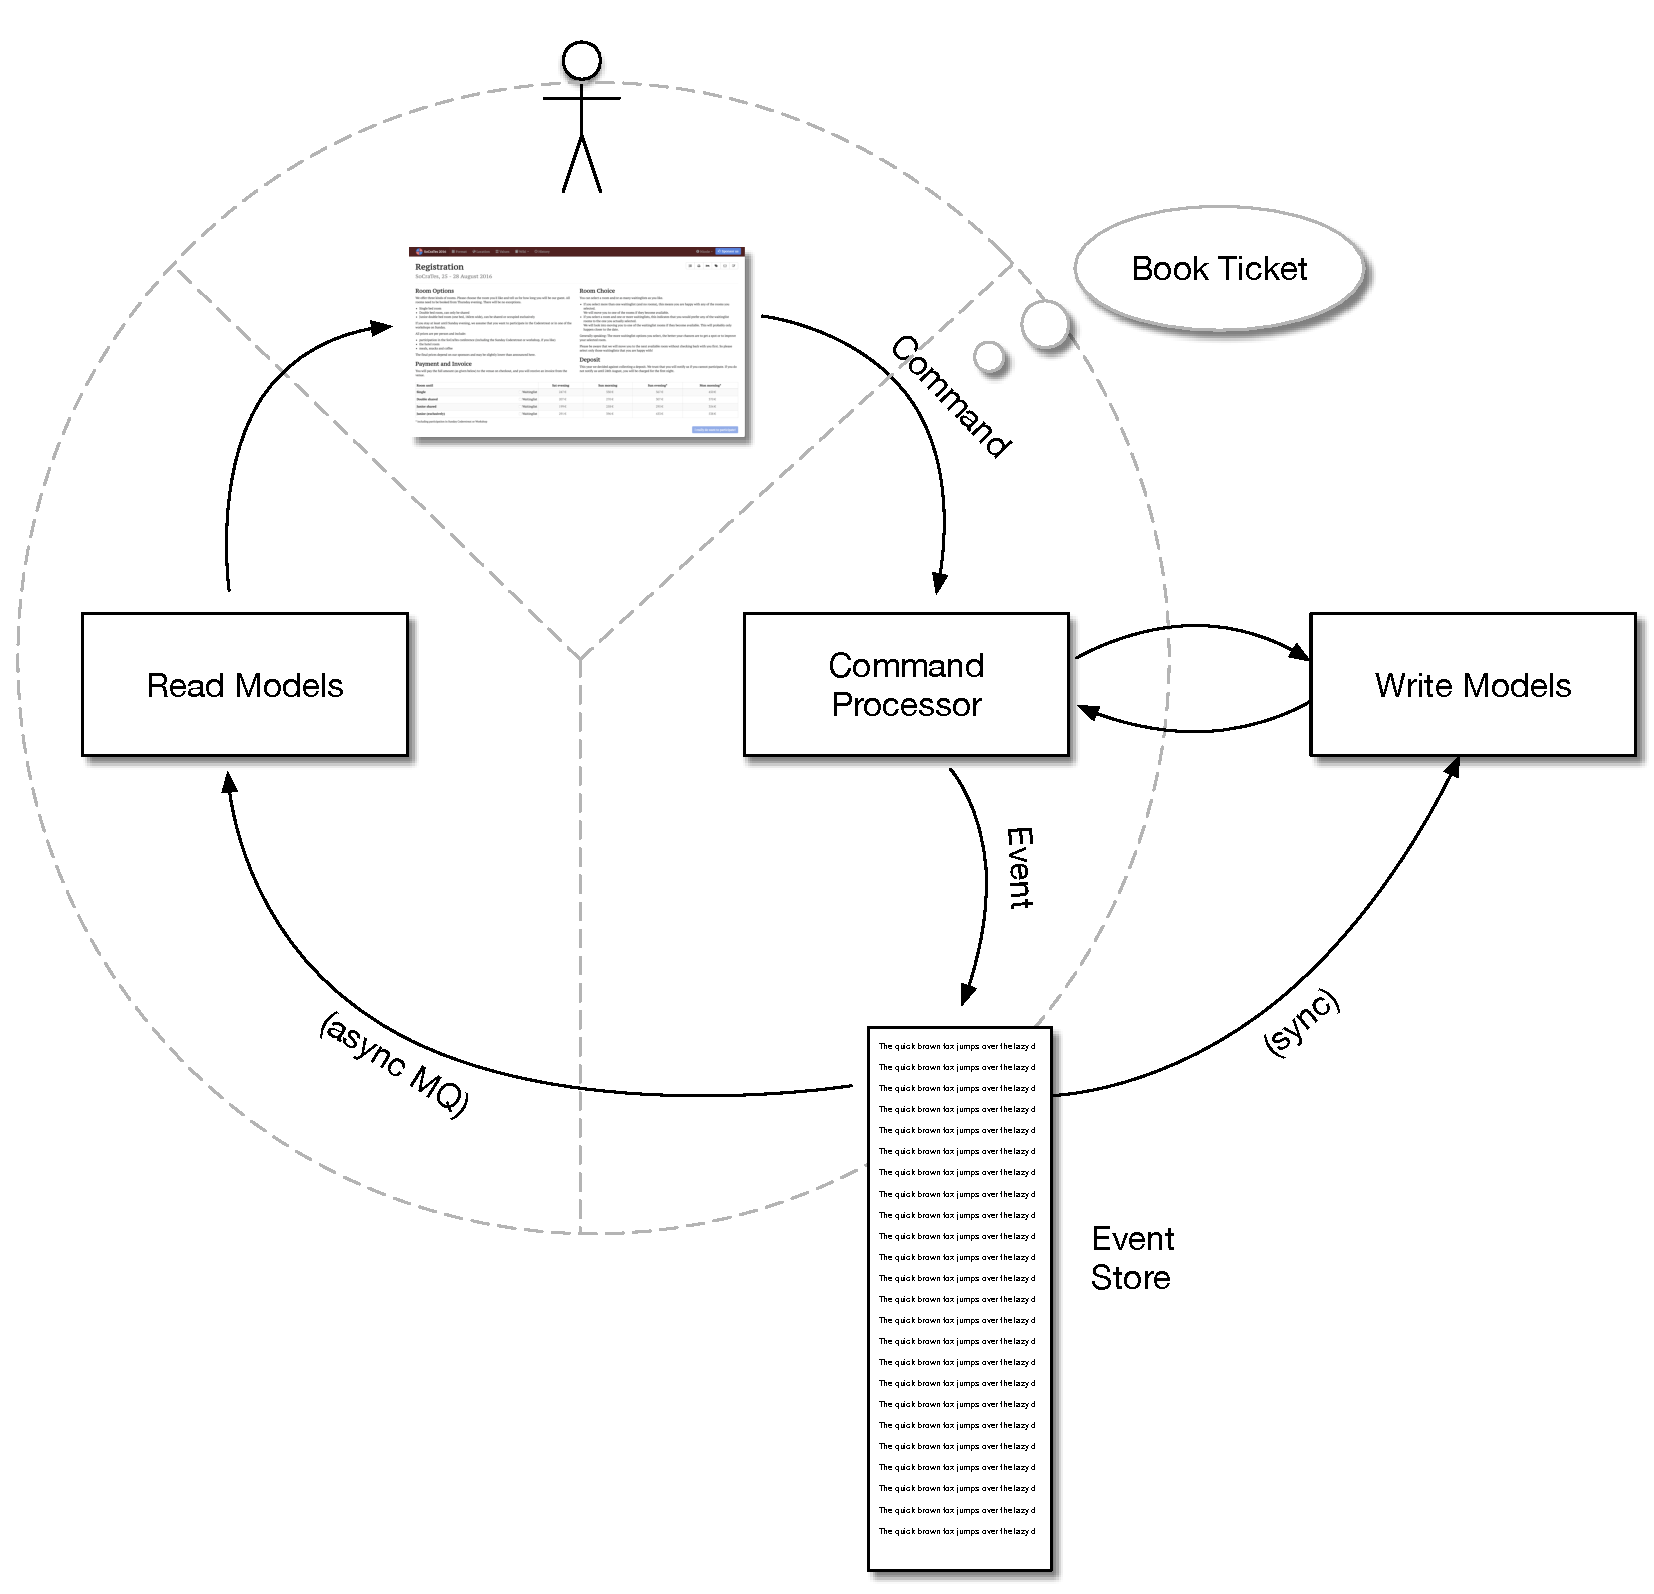
\includegraphics[width=.7\textwidth]{../EventSourcing4.pdf}
\end{onlyenv}

\begin{onlyenv}<2>
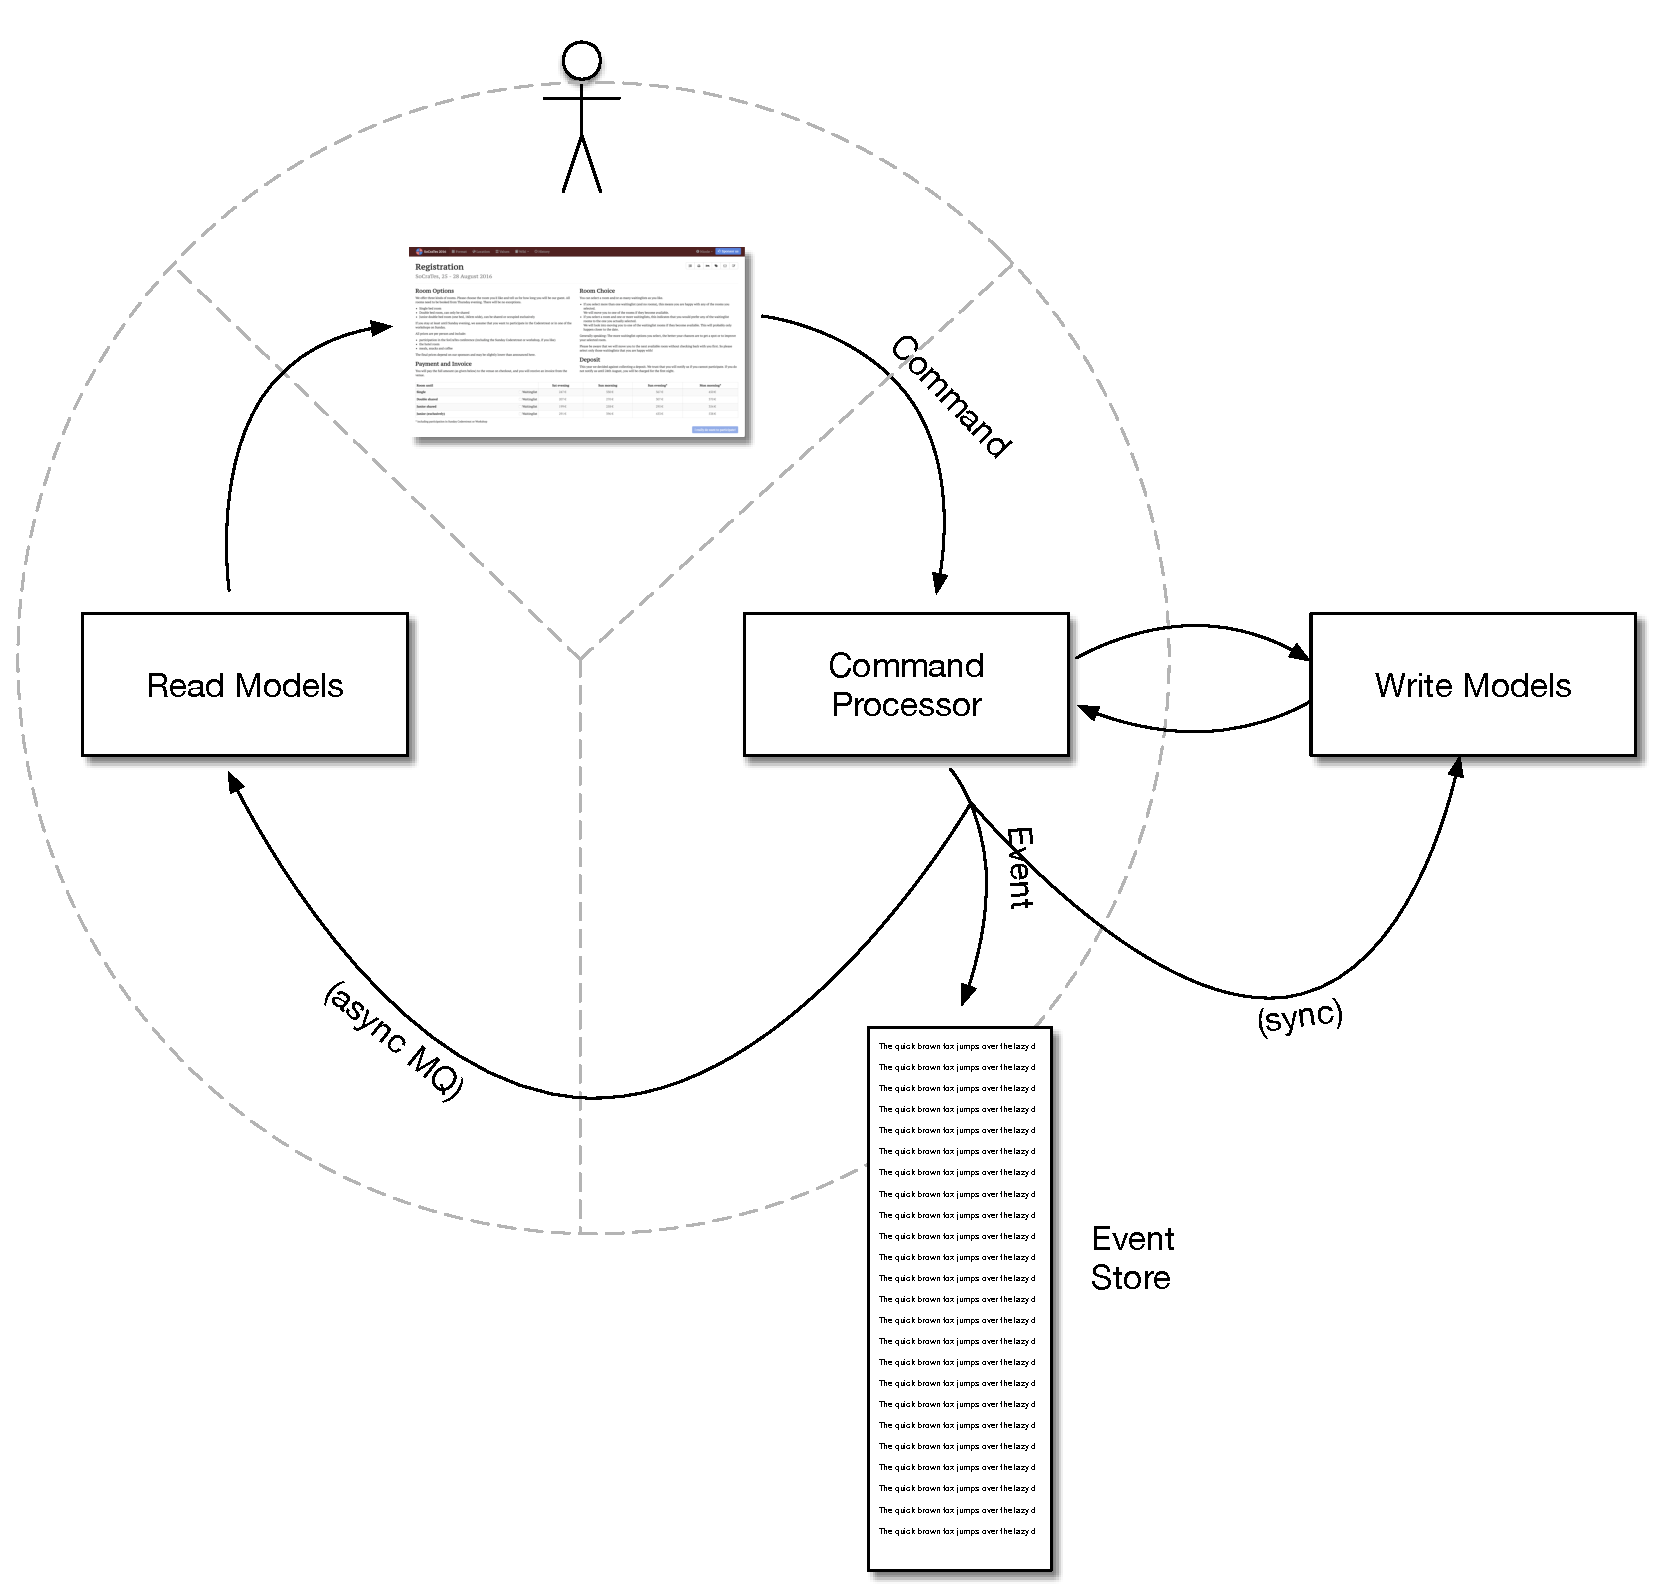
\includegraphics[width=.7\textwidth]{../EventSourcingOurStyle.pdf}
\end{onlyenv}


\begin{onlyenv}<3>

\textbf{Important:}

\vspace{4em}
Persisting the event store must be the \textbf{last} action to avoid parallelization!
\end{onlyenv}

\end{frame}

%%%%%%%%%%%%%%%%%%%%%%%%%%%%%%%%%%%%%%%%%%%%%%%%%%
\begin{frame}[fragile]{Caching Read and Write Models: The Read Models}

\renewcommand{\SPACE}{-0.9em}

\onslide+<1->
\begin{highlight}{1}
function getReadModel(url, key, ReadModel, callback) {
\end{highlight}
%%
\onslide+<2->
\vspace{\SPACE}
\begin{highlight}{2}
  const cacheKey = keyFor(url, key);
  var cachedModel = cache.get(cacheKey);
  if (cachedModel) {
    return callback(null, cachedModel);
  }
\end{highlight}
%%
\onslide+<3->
\vspace{\SPACE}
\begin{highlight}{3}
  eventstore.getEventStore(url, function (err, eventStore) {
    if (err || !eventStore) { return callback(err); }
\end{highlight}
%%
\onslide+<4->
\vspace{\SPACE}
\begin{highlight}{4}
    var cachedModel2 = cache.get(cacheKey);
    if (cachedModel2) {
      return callback(null, cachedModel2);
    }
\end{highlight}
%%
\onslide+<5->
\vspace{\SPACE}
\begin{highlight}{5}
    const newModel = new ReadModel(eventStore);
    cache.set(cacheKey, newModel);
    callback(null, newModel);
\end{highlight}
%%
\onslide+<3->
\vspace{\SPACE}
\begin{highlight}{3}
  });
\end{highlight}
%%
\onslide+<1->
\vspace{\SPACE}
\begin{highlight}{1}
}
\end{highlight}

\end{frame}

%%%%%%%%%%%%%%%%%%%%%%%%%%%%%%%%%%%%%%%%%%%%%%%%%%
\begin{frame}[fragile]{Caching Read and Write Models: The Write Models}

\renewcommand{\SPACE}{-0.9em}

\onslide+<1->
\begin{highlight}{1}
function getRegistrationCommandProcessor(url, callback) {
\end{highlight}
%%
\onslide+<2->
\vspace{\SPACE}
\begin{highlight}{2}
  getGlobalEventStoreForWriting(url, function (err, eventStore) {
    if (err || !eventStore) { return callback(err); }
\end{highlight}
%%
\onslide+<3->
\vspace{\SPACE}
\begin{highlight}{3}
    getReadModel(url, REGISTRATION_READ_MODEL, RegistrationReadModel, function (err1, registrationReadModel) {
      if (err1 || !registrationReadModel) { return callback(err1); }
\end{highlight}
%%
\onslide+<4->
\vspace{\SPACE}
\begin{highlight}{4}
      callback(null, new RegistrationCommandProcessor(new RegistrationWriteModel(eventStore, registrationReadModel)));
\end{highlight}
%%
\onslide+<3->
\vspace{\SPACE}
\begin{highlight}{3}
    });
\end{highlight}
%%
\onslide+<2->
\vspace{\SPACE}
\begin{highlight}{2}
  });
\end{highlight}
%%
\onslide+<1->
\vspace{\SPACE}
\begin{highlight}{1}
}
\end{highlight}

\onslide+<5->

Another deviation: WriteModel uses ReadModel

\end{frame}



%%%%%%%%%%%%%%%%%%%%%%%%%%%%%%%%%%%%%%%%%%%%%%%%%%
\begin{frame}[fragile]{Problem II}

\begin{itemize}
\item Parallelization due to database accesses
\item Large windows of parallelization due to slow request processing
\item Result: Write conflicts
\end{itemize}

\onslide+<2->
                  
\vspace{3em}

$\Longrightarrow$ We must eliminate write conflicts.
                  
\end{frame}

%%%%%%%%%%%%%%%%%%%%%%%%%%%%%%%%%%%%%%%%%%%%%%%%%%
\begin{frame}[fragile]{Controlling Parallelization}

\begin{center}

\begin{onlyenv}<1>
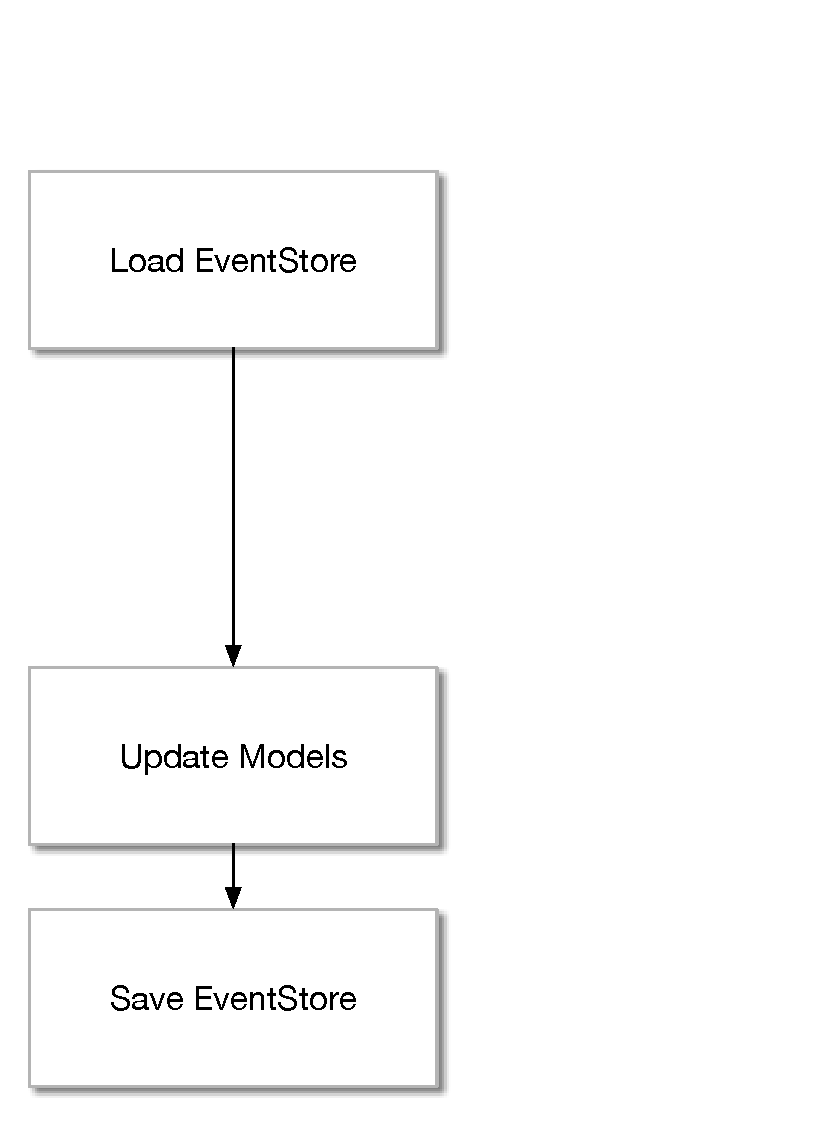
\includegraphics[width=.45\textwidth]{../EliminateWriteConflicts1.pdf}
\end{onlyenv}

\begin{onlyenv}<2>
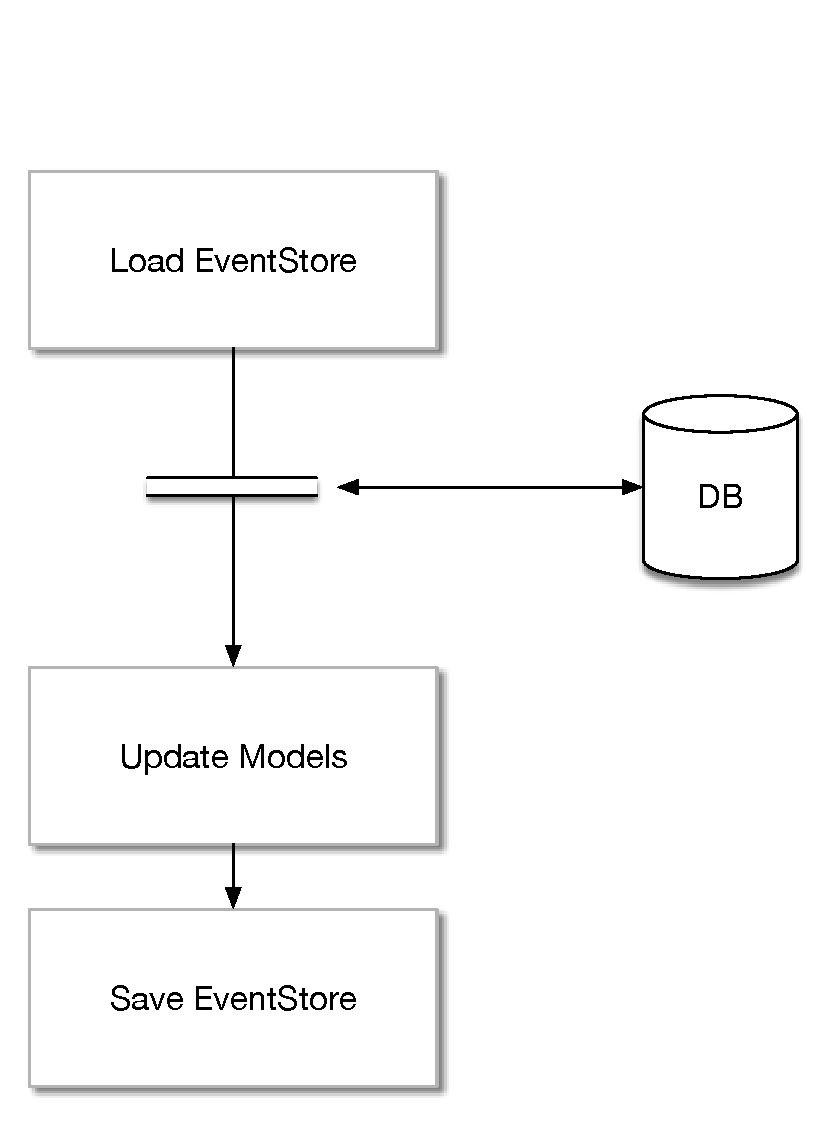
\includegraphics[width=.45\textwidth]{../EliminateWriteConflicts2.pdf}
\end{onlyenv}

\begin{onlyenv}<3>
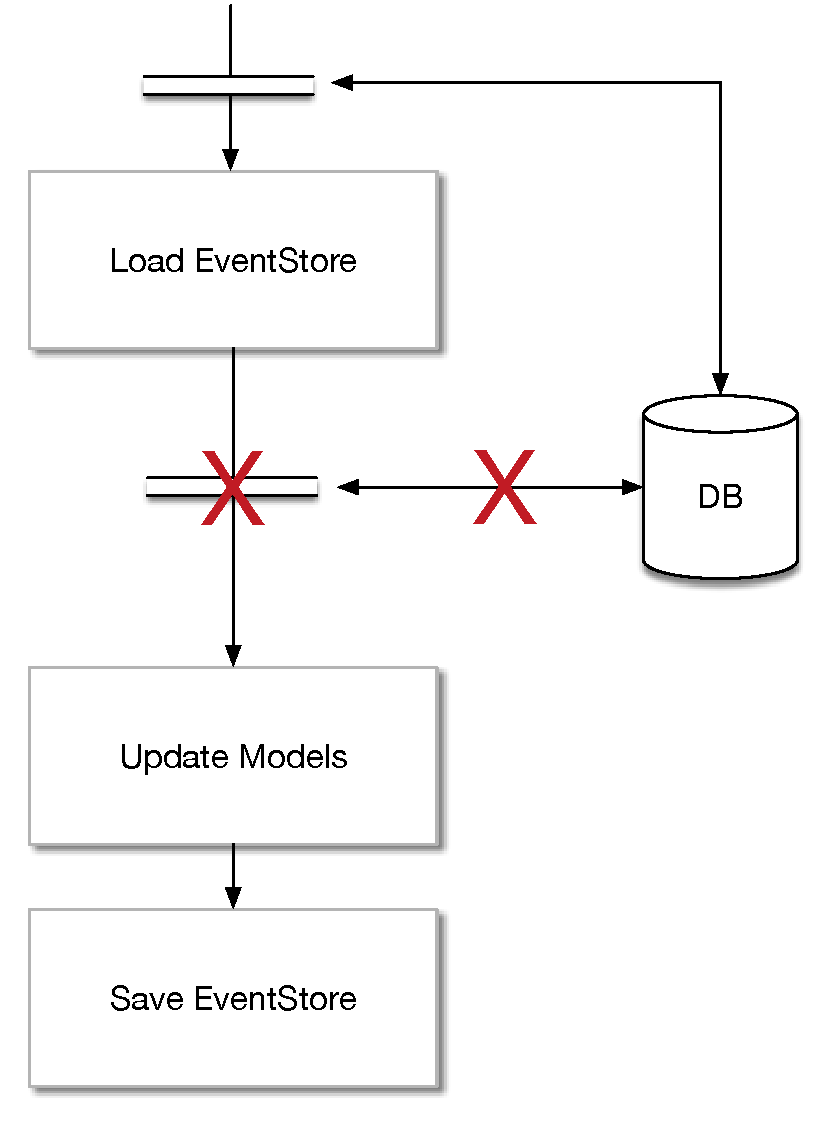
\includegraphics[width=.45\textwidth]{../EliminateWriteConflicts3.pdf}
\end{onlyenv}

\end{center}

\end{frame}


%%%%%%%%%%%%%%%%%%%%%%%%%%%%%%%%%%%%%%%%%%%%%%%%%%
\begin{frame}[fragile]{Benefits}

Synchronous code between loading and updating the event store

\onslide+<2->
\vspace{2em}

$\Longrightarrow$ No possibility for write conflicts

\onslide+<3->
\vspace{2em}

$\Longrightarrow$ We can even save unconditionally

\onslide+<4->
\vspace{2em}

$\Longrightarrow$ Event store is rather a backup

\end{frame}

%%%%%%%%%%%%%%%%%%%%%%%%%%%%%%%%%%%%%%%%%%%%%%%%%%
\begin{frame}[fragile]{Tradeoffs}

We cannot run multiple node.js processes in parallel

\onslide+<2->
\vspace{2em}

$\Longrightarrow$ No way of scaling

\end{frame}


%%%%%%%%%%%%%%%%%%%%%%%%%%%%%%%%%%%%%%%%%%%%%%%%%%
\begin{frame}{Thank you very much!}

        Slides: \url{https://github.com/NicoleRauch/EventSourcingNodeJS} 
        \vspace{1em}

        Code: \url{https://github.com/softwerkskammer/Agora}
        
        ~\\[1em]
        \begin{block}{Nicole Rauch}
        \begin{description}[Twitterxx]
                \item[E-Mail]  \href{mailto:info@nicole-rauch.de}{\texttt{info@nicole-rauch.de}}
                \item[Twitter] \href{http://twitter.com/NicoleRauch}{\texttt{@NicoleRauch}}
                \item[Web] \href{http://www.nicole-rauch.de}{\texttt{http://www.nicole-rauch.de}}
        \end{description}
        \end{block}
\end{frame}

